\documentclass[ALICE,manyauthors]{cernphprep}

\usepackage[comma,square,numbers,sort&compress]{natbib}
\usepackage{hyperref}
\usepackage{lineno}
\usepackage{subfigure}
\usepackage[section]{placeins}
\usepackage {multicol}% Multi column in the table
\usepackage {multirow}% Multi row in the table
\usepackage {units}
\usepackage {array}
\usepackage {xcolor}
\usepackage{comment}
\linenumbers

% $Id: commands.tex 934 2013-06-19 20:56:45Z mfloris $

\newcommand{\mrm}[1]{\mathrm{#1}}
\newcommand{\mrmo}[1]{\mathrm{\overline{#1}}}
\newcommand{\bsb}[1]{\boldsymbol{#1}}
\newcommand{\circit}{\item[$\circ$]}


\newcommand{\fzero}{$\mathrm{f}_{0} (980)$}
\newcommand{\ITS}          {\rm{ITS}}
\newcommand{\TOF}          {\rm{TOF}}
\newcommand{\ZDC}          {\rm{ZDC}}
\newcommand{\ZDCs}         {\rm{ZDCs}}
\newcommand{\ZNA}          {\rm{ZNA}}
\newcommand{\ZNC}          {\rm{ZNC}}
\newcommand{\SPD}          {\rm{SPD}}
\newcommand{\SDD}          {\rm{SDD}}
\newcommand{\SSD}          {\rm{SSD}}
\newcommand{\TPC}          {\rm{TPC}}
\newcommand{\VZERO}        {\rm{VZERO}}
\newcommand{\VZEROA}       {\rm{VZERO-A}}
\newcommand{\VZEROC}       {\rm{VZERO-C}}
\newcommand{\pip}          {$\pi^{+}$}
\newcommand{\pim}          {$\pi^{-}$}
\newcommand{\kap}          {K$^{+}$}
\newcommand{\kam}          {K$^{-}$}
\newcommand{\pbar}         {$\rm\overline{p}$}
\newcommand{\kzero}        {\ensuremath{{\rm K}^{0}_{S}}}
\newcommand{\kstar}        {\ensuremath{{\rm K}^{*}}}
\newcommand{\He}           {\ensuremath{^{3}{\rm He}}}
\newcommand{\LH}           {\ensuremath{^{3}_{\Lambda}{\rm H}}}
\newcommand{\vzero}        {\ensuremath{{\rm V}^0}}
\newcommand{\lmb}          {\ensuremath{\Lambda}}
\newcommand{\almb}         {\ensuremath{\bar{\Lambda}}}
\newcommand{\allpart}      {$\pi^{\pm}$, K$^{\pm}$, \kzero, p(\pbar) and \lmb(\almb)}
\newcommand{\allpi}        {$\pi^{\pm}$}
\newcommand{\allk}         {K$^{\pm}$}
\newcommand{\allp}         {p(\pbar)}
\newcommand{\alllmb}       {\lmb(\almb)}
\newcommand{\degree}       {$^{\rm o}$}
\newcommand{\dg}           {\mbox{$^\circ$}}
\newcommand{\dedx}         {\ensuremath{\mathrm{d}E/\mathrm{d}x}}
\newcommand{\dndy}         {d$N$/d$y$}
\newcommand {\ee}            {\mbox{e$^+$e$^-$}}
\newcommand{\pp}           {pp}
\newcommand{\ppbar}        {\mbox{$\mathrm {p\overline{p}}$}}
\newcommand{\PbPb}         {\mbox{Pb--Pb}}
\newcommand{\pPb}          {\mbox{p--Pb}}
\newcommand{\AuAu}         {\mbox{Au--Au}}
\newcommand{\pseudorap}    {\mbox{$\left | \eta \right | $}}
\newcommand{\dNdeta}       {\ensuremath{\mathrm{d}N_\mathrm{ch}/\mathrm{d}\eta}}
\newcommand{\dNdy}         {\ensuremath{\mathrm{d}N/\mathrm{d}y}}
\newcommand{\dNdptdy}      {\ensuremath{\mathrm{d}N/{\rm d}\pt\mathrm{d}y}}
\newcommand{\dNdyst}       {\ensuremath{\sqrt{\frac{dN_\pi/dy}{s_T}}}}
\newcommand{\dNdetatr}     {\mathrm{d}N_\mathrm{tracklets}/\mathrm{d}\eta}
\newcommand{\dNdetar}[1]   {\mathrm{d}N_\mathrm{ch}/\mathrm{d}\eta\left.\right|_{|\eta|<#1}}
\newcommand{\lum}          {\, \mbox{${\rm cm}^{-2} {\rm s}^{-1}$}}
\newcommand{\barn}         {\, \mbox{${\rm barn}$}}
\newcommand{\m}            {\, \mbox{${\rm m}$}}
\newcommand{\ncls}         {\ensuremath{N_{cls}}}
\newcommand{\nsigma}       {\ensuremath{n\sigma}}
\newcommand{\dcaxy}        {\ensuremath{{\rm DCA}_{xy}}}
\newcommand{\dcaz}         {\ensuremath{{\rm DCA}_{z}}}
\newcommand{\EcrossB}      {E$\times$B}%{\ensuremath{{\rm E}\times{\rm B}}}
\newcommand{\bb}           {Bethe-Bloch}
\newcommand{\s}            {\ensuremath{\sqrt{s}}}
\newcommand{\pt}           {\ensuremath{p_\mathrm{T}}}
\newcommand{\pT}           {\ensuremath{p_{\rm T}}}
\newcommand{\hlab}         {\ensuremath{\eta_{\rm lab}}}
\newcommand{\ynn}         {\ensuremath{y_{\rm NN}}}
\newcommand{\ycms}         {\ensuremath{y_{\rm CMS}}}
\newcommand{\ylab}         {\ensuremath{y_{\rm lab}}}
\newcommand{\ppi}          {\ensuremath{{\rm p}/\pi}}
\newcommand{\kpi}          {\ensuremath{{\rm K}/\pi}}
\newcommand{\lpi}          {\ensuremath{{\rm \Lambda}/\pi}}
%\newcommand{\ppi}          {\ensuremath{(\pi^+ + \pi^-)/({\rm K}^+ + {\rm K}^-)}}
%\newcommand{\kpi}          {\ensuremath{({\rm p} + {\rm \bar p})/({\rm K}^+ + {\rm K}^-)}}
\newcommand{\mt}           {\ensuremath{m_{\rm T}}}
\newcommand{\snn}          {\ensuremath{\sqrt{s_{\rm NN}}}}
\newcommand{\snnbf}        {\ensuremath{\mathbf{{\sqrt{s_{\mathbf NN}}}}}}
\newcommand{\sonly}        {\ensuremath{\sqrt{s}}}
\newcommand{\Npart}        {\ensuremath{N_\mathrm{part}}}
\newcommand{\avNpart}      {\ensuremath{\langle N_\mathrm{part} \rangle}}
\newcommand{\avNpartdata}  {\ensuremath{\langle N_\mathrm{part}^{\rm data} \rangle}}
\newcommand{\Ncoll}        {\ensuremath{N_\mathrm{coll}}}
\newcommand{\Dnpart}       {\ensuremath{D\left(\Npart\right)}}
\newcommand{\DnpartExp}    {\ensuremath{D_{\rm exp}\left(\Npart\right)}}
\newcommand{\dNdetapt}     {\ensuremath{\dNdeta\,/\left(0.5\Npart\right)}}
\newcommand{\dNdetaptr}[1] {\ensuremath{\dNdetar{#1}\,/\left(0.5\Npart\right)}}
\newcommand{\dNdetape}     {\left(\ensuremath{\dNdeta\right)/\left(\avNpart/2\right)}}
\newcommand{\dNdetaper}[1] {\ensuremath{\dNdetar{#1}\,/\left(\avNpart/2\right)}}
\newcommand{\dndydpt}      {\ensuremath{{\rm d}^2N/({\rm d}y {\rm d}p_{\rm t})}}
\newcommand{\abs}[1]       {\ensuremath{\left|#1\right|}}
\newcommand{\signn}        {\ensuremath{\sigma^{\rm inel.}_{\rm NN}}}
\newcommand{\vz}           {\ensuremath{V_{z}}}
\newcommand{\Tfo}          {\ensuremath{{T}_{\rm kin}}}
\newcommand{\Tch}          {\ensuremath{{T}_{\rm ch}}}
\newcommand{\bT}           {\ensuremath{\beta_{\rm T}}}
\newcommand{\avbT}         {\ensuremath{\left< \beta_{\rm T}\right>}}
\newcommand{\avpT}         {\ensuremath{\left< \pt \right>}}
\newcommand{\muB}          {\ensuremath{\mu_{B}}}
\newcommand{\stat}         {({\it stat.})}
\newcommand{\syst}         {({\it sys.})}
\newcommand{\Fig}[1]       {Fig.~\ref{#1}}
\newcommand{\Figure}[1]    {Figure~\ref{#1}}
%\newcommand{\Ref}[1]       {Ref.~\cite{#1}}
%\newcommand{\green}[1]     {\textcolor{green}{#1}}
%\newcommand{\blue}[1]      {\textcolor{blue}{#1}}
%\newcommand{\red}[1]       {\textcolor{red}{#1}}
%\newcommand{\white}[1]     {\textcolor{white}{#1}}
\newcommand{\gevc}         {\ensuremath{{\rm GeV}/c}}
\newcommand{\mevc}         {\ensuremath{{\rm MeV}/c}}
\newcommand{\gs}           {\ensuremath{\gamma_{s}}}
\newcommand{\gq}           {\ensuremath{\gamma_{q}}}
\newcommand{\gc}           {\ensuremath{\gamma_{c}}}
\newcommand{\chindf}       {\ensuremath{\chi^{2}/{\rm NDF}}}
\newcommand{\avg}[1]       {\ensuremath{\left\langle#1\right\rangle}}
\newcommand{\etalab}       {\ensuremath{\eta_{{\rm lab}}}}
\newcommand {\gammas}			{\ensuremath{\gamma_{\mathrm{s}}}}

\newcommand{\DNDETAINEL}{5.31~$\pm$~0.18\xspace}
\newcommand{\DNDETAINELGTZERO}{6.46~$\pm$~0.19\xspace}
\newcommand{\DNDETAINELGTZEROONE}{6.61~$\pm$~0.20\xspace}

\newcommand{\inelgtzero}{INEL$>$0\xspace}
\newcommand{\average}[1]{\ensuremath{\langle #1 \rangle}\xspace}
\newcommand{\mpt}        {\ensuremath{\langle\pt\rangle}\xspace}
\newcommand{\nch}        {\ensuremath{N_\mathrm{ch}}\xspace}
\newcommand{\mnch}      {\ensuremath{\langle\nch\rangle}\xspace}
\newcommand{\nchacc}        {\ensuremath{N_\mathrm{ch}^\mathrm{acc}}\xspace}
\newcommand{\mnchacc}      {\ensuremath{\langle\nchacc\rangle}\xspace}
\newcommand{\inelg}     {\ensuremath{\mathrm{INEL}_{>0}}}



\newcommand{\dndeta}{\ensuremath{{\rm d}N_{\rm ch}/{\rm d}\eta}\xspace}
\newcommand{\dndpt}{\ensuremath{{\rm d}N_{\rm ch}/{\rm d}\pt}\xspace}
\newcommand{\etaless}[1]{\ensuremath{\left|\eta\right| < #1}\xspace}
\newcommand{\dndetaless}[1]{\ensuremath{{\rm d}N_{\rm ch}/{\rm d}\eta|_{\etaless{#1}}}\xspace}
\newcommand{\avdndeta}{\ensuremath{\langle \dndeta \rangle}}
\newcommand{\zvtx}{\ensuremath{z_\mathrm{vtx}}}
\newcommand{\pythiae}{\ensuremath{\mathrm{PYTHIA}\,8}}
%\newcommand{\pythiam}{\ensuremath{\mathrm{PYTHIA}\,8\,\mathrm{Monash}\,2013}}
\newcommand{\pythiam}{\ensuremath{\mathrm{PYTHIA}\,8\,\mathrm{Tune\,4C}}}
\newcommand{\pythiashoving}{{\ensuremath{\mathrm{PYTHIA}\,8~\mathrm{String}~}}\ensuremath{\mathrm{Shoving}}}
\newcommand{\epos}{{\ensuremath{\mathrm{EPOS}\,~\mathrm{LHC}}}}
%\newcommand{\pythiashoving}{\ensuremath{\mathrm{PYTHIA}\,8~\mathrm{String}~}\linenomath{-}\ensuremath{\mathrm{Shoving}}}
\newcommand{\pttrig}{\ensuremath{p_\mathrm{T,\,trig}}}
\newcommand{\ptassoc}{\ensuremath{p_\mathrm{T,\,assoc}}}
\newcommand{\ptjet}{\ensuremath{p_\mathrm{T,\,jet}^\mathrm{ch}}}
\newcommand{\ptlead}{\ensuremath{p_\mathrm{T,\,LP}}}
\newcommand{\pttrigassoc}{\ensuremath{p_\mathrm{T,\,trig\,(assoc)}}}
\newcommand{\qppb}{\ensuremath{Q_{\mbox{p--Pb}}}}









\renewcommand{\labelitemi} {$-$}
%==========================================================%
%%% inline warnings for internal discussion
%\newcommand{\warn}[1]      {\textbf{\textcolor{red}{[#1]}}}
\newcommand{\warn}[1]      {{\small\textbf{\textcolor{red}{(!\footnote{\textbf{(!)}~#1})}}}}
\newcommand{\warnin}[1]         {\textit{\textcolor{red}{(#1)}}}
%\newcommand{\warn}[1]      {#1}
%\newcommand{\warn}[1]      {{\small\textbf{(!\footnote{\textbf{(!)}~#1})}}\marginpar{\textbf{---}}}
\newcommand{\todo}[1]      {\textbf{\textcolor{red}{[TODO: #1]}}}
%%% fake numbers
\newcommand{\fake}[1]      {\textbf{\textcolor{red}{#1}}}
%\newcommand{\fake}[1]      {#1}
\newcommand{\final}[1]     {\textbf{\textcolor{blue}{#1}}}
\newcommand{\prelim}[1]    {\textbf{\textcolor{magenta}{#1}}}
\renewcommand{\mod}[1]       {\textbf{\textcolor{red}{#1}}}

\begin{document}

%%%%%%%%%%%%%%%  Title page %%%%%%%%%%%%%%%%%%%%%%%%
\begin{titlepage}

\PHyear{}
\PHnumber{2021-xxx}      % required, will be obtained from PH
%\PHdate{Day Month}  % required, will be obtained from PH
\PHdate{\today}
%

%%% Put your own title + short title here:
\title{Observation of abnormal suppression of $\mathrm{f}_{0}$(980) production \\in p--Pb collisions at $\snn$ = 5.02~TeV }

\ShortTitle{}   % appears on right page headers

%%% Do not change the next lines
%\Collaboration{ALICE Collaboration\thanks{See Appendix~\ref{app:collab} for the list of collaboration members}}
\ShortAuthor{ALICE Collaboration} % appears on left page headers, do not change

\begin{abstract}
The multiplicity dependence of $\mathrm{f}_{0}$(980) production in p--Pb collisions at $\sqrt{s_{\mathrm{NN}}} = 5.02$~TeV with ALICE is reported. The production of $\mathrm{f}_{0}$(980) is measured via the $\mathrm{f}_0 (980) \rightarrow \pi^{+}\pi^{-}$ decay channel in a midrapidity region of $-0.5<y<0$. Particle yield ratios of $\mathrm{f}_{0}$(980) to $\pi$ and \kstar~are found to be decreasing with an increasing charged-particle multiplicity. The yield ratios of $\mathrm{f}_{0}$(980) as a function of its transverse momentum ($p_{\mathrm{T}}$) exhibit a particle-species-dependent behavior. Furthermore, the nuclear modification factor $Q_{\mbox{pPb}}$ ($R_{\mbox{pPb}}$ in centrality intervals, due to the possible bias in the determination of centrality) is measured in various multiplicity ranges. The $Q_{\mbox{pPb}}$ shows strong suppression in the  $p_{\mathrm{T}}$ region up to about 4~GeV/$c$. The results of the particle yield ratios and $Q_{\mbox{pPb}}$ for $\mathrm{f}_{0}$(980) may help to understand the late hadronic phase in p--Pb collisions and the nature of the internal structure of $\mathrm{f}_{0}$(980) particles.



\color{black}

\end{abstract}
 
\end{titlepage}

\setcounter{page}{2}

% !TEX root = paper.tex

\section{Introduction}

Light scalar mesons, whose spin and parity are zero and even, respectively, are of particular interest as their nature can be explained with an exotic structure~\cite{ParticleDataGroup:2022pth}. Among them, the understanding of \fzero\ particle lies in a long-standing puzzle in terms of its quark content~\cite{ExHIC:2010gcb, Jaffe:1976ig, Maiani:2004uc}. The \fzero\ is suggested to be a conventional $\rm{}q\bar{q}$~\cite{Chen:2003za}, compact tetraquark~\cite{Achasov:2020aun}, or $\rm{}K\overline{K}$ molecule~\cite{Ahmed:2020kmp}. In order to analyze the unknown structure of \fzero, several approaches are accessible in relativistic heavy-ion collisions in conjunction with the information in proton--proton (pp) collisions. 

The theory of strong interaction, quantum chromodynamics (QCD), predicts the formation of a state of strongly interacting matter, the so called quark-gluon plasma (QGP), in the hot and dense system reached in relativistic heavy-ion collisions. Many observations at the Large Hadron Collider (LHC), such as flow modulations~\cite{Bhalerao:2020ulk, ALICE:2019zfl}, jet quenching~\cite{ALICE:2019qyj}, and nuclear modification factors~\cite{ALICE:2019hno}, support the existence of the QGP~\cite{Adams:2005dq}. Specifically, the nuclear modification factors for different particle species in heavy-ion collisions show that the transverse momentum ($p_{\mathrm{T}}$) distribution of particles is strongly modified due to the presence of the hot and dense QGP medium. However, the nuclear modification factors are measured as close to unity in p--A collisions~\cite{ALICE:2016dei} for minimum-bias (MB) events, stating no substantial modification in p--A collisions in the high $p_{\mathrm{T}}$ range~($>$~8~GeV/$c$). 

The relative production yield of particles containing strange quarks is reported to increase faster than those with up and down quarks, which is usually referred to as ``strangeness enhancement''~\cite{ALICE:2016fzo} in high-multiplicity pp and p--Pb collisions. The observation of the strangeness enhancement, along with measurements of flow modulations in small collision systems~\cite{PHENIX:2018lia, ALICE:2021nir}, may hint at the formation of QGP droplets in small systems. The study of relative production yield for \fzero\ can be helpful to check the strange quark content~\cite{LHCb:2014ooi, LHCb:2014vbo} inside \fzero. On the other hand, the nuclear modification factors for baryons exhibit a strong enhancement at intermediate $p_{\mathrm{T}}$ (2~$<p_{\mathrm{T}}<$~5~GeV/$c$) compared with those for mesons, which is mainly due to the number of constituent quarks (NCQ)~\cite{Cronin:1974zm, Fries:2003vb}. In addition, it has been suggested that the elliptic flows of different particles depend on the NCQ, as demonstrated in Ref.~\cite{Wang:2022det}. These approaches can help to constrain the number of quarks forming \fzero.

The short-lived resonances, such as \rhoz~\cite{ALICE:2018qdv}, \kstar~\cite{ALICE:2019etb, ALICE:2016sak}, $\Sigma(1385)^{\pm}$~\cite{ALICE:2022zuc}, and $\Lambda$(1520)~\cite{ALICE:2018ewo} as well as \fzero, are good probes to study the properties of the system that results from the hadronization of a QGP~\cite{Bierlich:2021poz}. In the late stage of the evolution of the system formed in heavy-ion collisions, there are two important temperatures and corresponding timescales: the chemical freeze-out, when the inelastic collisions among the constituents are expected to cease, and the later kinetic freeze-out, when all (elastic) interactions stop~\cite{Song:1996ik}. Because the duration between the chemical to the kinetic freeze-outs of the system is comparable with the lifetime of resonances~\cite{ALICE:2011dyt, ALICE:2019xyr}, their decay products can actively interact with the hadronic gas via rescattering and regeneration processes, and such interactions result in modifications of resonance yields. The modifications can be observed by comparing the yield of resonances with those of long-lived or ground-state particles~\cite{ALICE:2018pal}. Measurements of \rhoz$/\pi$ and \kstar$\rm{}/K$ yield ratios are good examples to study the properties of the late hadronic phase after the chemical freeze-out. Recently, system-size-dependent suppressions of particle yields are also observed in small systems~\cite{ALICE:2019etb}, suggesting rescattering and regeneration processes in small systems. Observing the modification for the \fzero~yield may contribute to further understanding the late hadronic phase.

In this paper, multiplicity-dependent measurement of anomalous suppression of \fzero~production in p--Pb collisions at $\snn$ = 5.02~TeV is reported for the first time. The measurement of \fzero~is conducted at midrapidity (-0.5~$<y<$~0) in 0~$<p_{\mathrm{T}}<$~8~GeV/$c$ for different multiplicity classes. In Sec.~\ref{sec:setup}, the experimental setup is described, while the reconstruction of \fzero\ and the relative corrections are explained in Sec.~\ref{sec:ana}. The study of systematic uncertainties for the measurement is reported in Sec.~\ref{sec:syst}. In Sec.~\ref{sec:results}, $p_{\mathrm{T}}$ spectra, particle yield ratios, and the nuclear modification factors are discussed. Finally, model comparisons and conclusions are described in Sec.~\ref{sec:summary}.

\label{sec:intro}




\section{Experimental setup}
\label{sec:setup}
The minimum-bias (MB) events in p--Pb collisions at $\snn$~=~5.02~TeV used for the present analysis are recorded by the ALICE detector in 2016. The nucleon–nucleon centre-of-mass system is shifted by $\Delta \mathrm{y}_{\mathrm{cms}} =$~0.465 in the unit of rapidity along the direction of the proton beam. The entire subsystem of the ALICE detector can be found in Ref.~\cite{Abelev:2014ffa} for the LHC Run 2 period. The present analysis is carried out with the Inner Tracking System (ITS)~\cite{ALICE:2010tia}, the Time Projection Chamber (TPC)~\cite{Alme:2010ke}, the Time-Of-Flight (TOF)~\cite{Jacazio:2018slq}, V0~\cite{ALICE:2013axi}, and the Zero Degree Calorimeter (ZDC)~\cite{Cortese:2019nnv}. 

The V0 detector has two stations located at both forward sides with respect to the nominal interaction point, V0A and V0C, each made of 32 plastic scintillator strips, covering the full azimuthal angle within the pseudorapidity intervals $2.8 < \eta < 5.1$ and $-3.7 < \eta < -1.7$, respectively. V0A detector on Pb-going side is used to provide a MB trigger in p--Pb collisions. The V0A provides the multiplicity class using the sum of the V0A signals at the same time. The collected data samples from the MB trigger correspond to the integrated luminosity of 0.24~nb$^{-1}$~\cite{ALICE:2014gvw}. The ZDC which detects ``slow'' nucleons at very large $\eta$~\cite{Cortese:2019nnv} also defines the most unbiased multiplicity class. The multiplicity of neutrons by nuclear de-excitation processes or neutrons knocked out from wounded nucleons is expected to increase with the number of nucleon–nucleon binary collisions at the Pb-going side~\cite{ALICE:2014xsp}. This multiplicity definition is the least-biased centrality estimator for p--Pb collisions.

%The V0A detector is utilized to measure the particle yield ratio of \fzero~because the multiplicity dependence of $\mathrm{K}^{*0}$ and $\pi$ yields are measured with the V0A detector. The ZDC which detects ``slow'' nucleons at very large $\eta$~\cite{Cortese:2019nnv}  also defines the most unbiased multiplicity class for the event selection. The multiplicity dependence of the nuclear modification factor of \fzero~is measured using the hybrid method, which can be conducted with the ZDC~\cite{ALICE:2014xsp}, to scale down the cross section of the \fzero~in p--Pb collisions with a reduced bias.

The primary vertex position is reconstructed using the measured track segments in the Silicon Pixel Detector (SPD)~\cite{Santoro2009:ALICESPD}, which is the innermost two layers of the ITS. The reconstructed primary vertex is required to be within 10~cm from the center of the detector along the beam direction. Pileup events are rejected when multiple primary vertices are reconstructed and the longitudinal displacement of their reconstructed vertices is larger than 0.8~cm. The probability of pileup events is expected to be 0.5\% in MB events. The TPC is the main tracking detector of ALICE, covering a pseudorapidity range $|\eta|<$~0.9 over the full azimuth in a uniform solenoidal magnetic field of 0.5~T along the beam axis. The TPC can reconstruct charged tracks originating from the primary vertex down to $p_{\rm{T}}=$~0.1~GeV/$c$. Particle identification (PID) can be done with the TPC and TOF. The TPC measures ionization energy loss $\mathrm{d}E/\mathrm{d}x$ of charged tracks to separate particle species. The TOF helps the PID capabilities of the TPC by measuring the flight time of charged particles from the interaction point to the TOF.

\section{Data analysis}
\label{sec:ana}
\begin{figure}[hbt!]
	\centering
	\subfigure{ 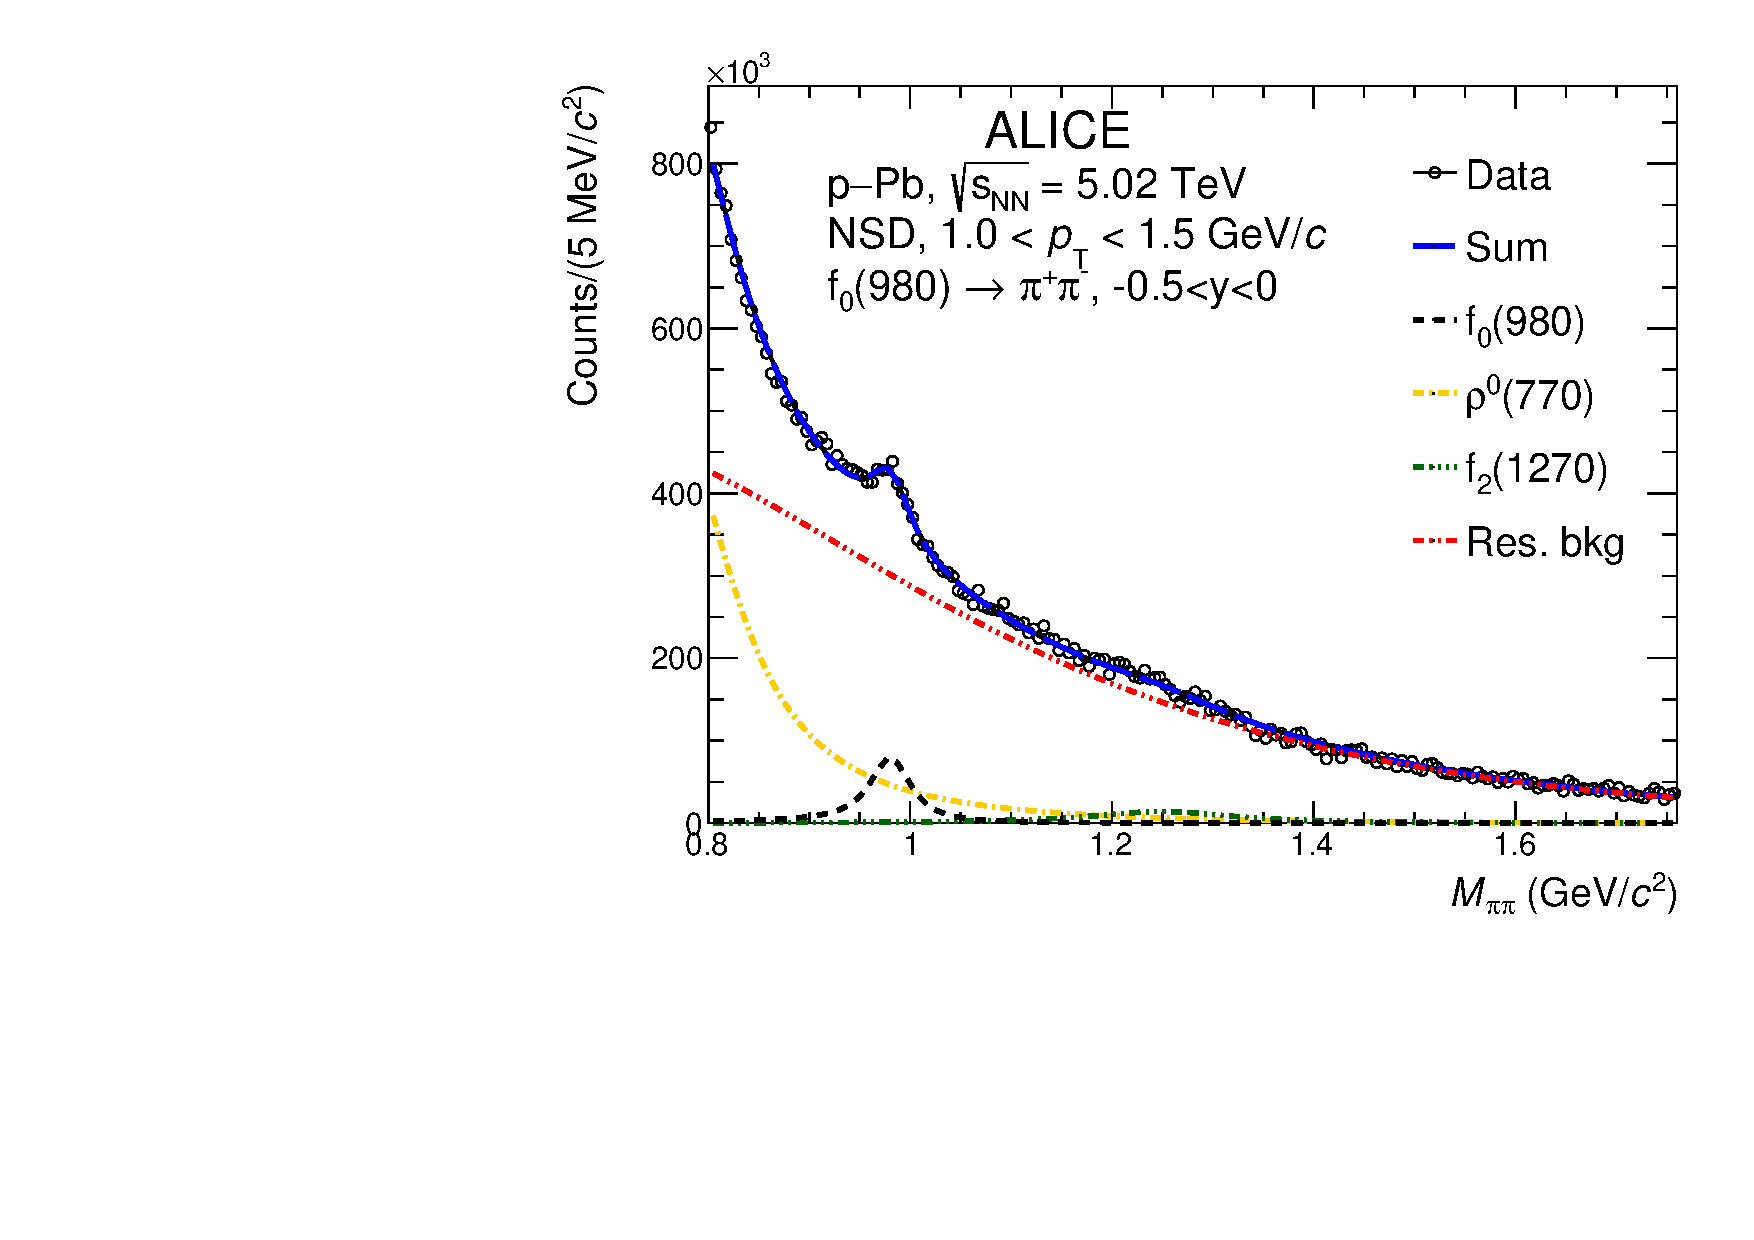
\includegraphics[width=0.47 \textwidth]{figures/Fig1_sigext_mb_0pt_mb.pdf} }
	\subfigure{ 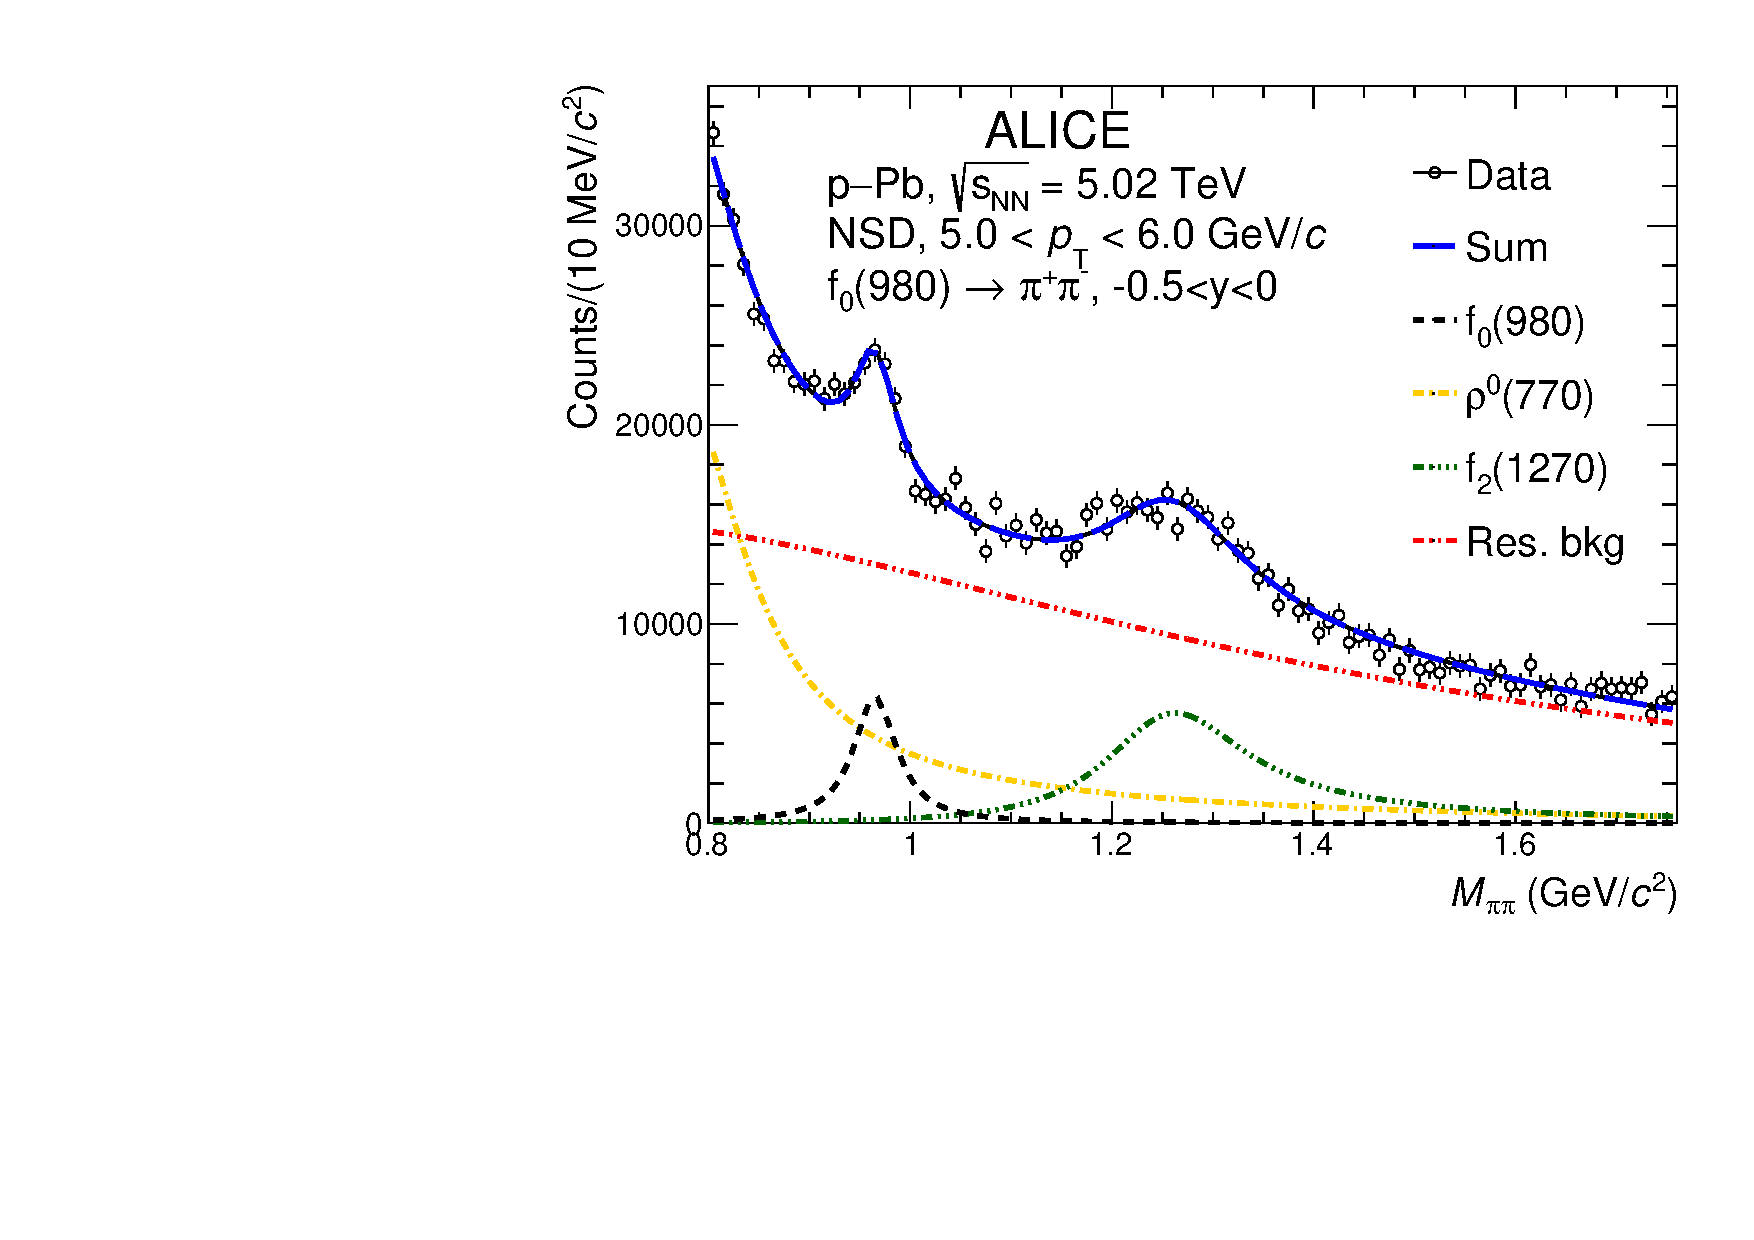
\includegraphics[width=0.47 \textwidth]{figures/Fig1_sigext_mb_1pt_mb.pdf} }
	\caption{ Invariant mass distribution of $\pi^{+}\pi^{-}$ pairs in -0.5~$<\mathrm{y}<$~0 after like-sign backgrounds subtraction in p--Pb collisions at \snn~=~5.02~TeV. The left (right) plot is obtained at low (high) $p_{\mathrm{T}}$ of $\pi^{+}\pi^{-}$ pairs in non-single diffraction (NSD) events }
	\label{fig:SigExt}
\end{figure}

The \fzero~is reconstructed with the decay channel of \fzero~$\rightarrow \pi^{+}\pi^{-}$, where the branching ratio of the decay is 46~$\pm$~6\%~\cite{Stone:2013eaa}. Each charged pion is required to have $p_{\rm{T}}>$~0.15~GeV/$c$ and $|\eta|<$~0.8 for a uniform detector acceptance. The reconstructed tracks are required to satisfy selection criteria listed in the previous work~\cite{ALICE:2018qdv} to guarantee the good reconstruction of charged tracks. In particular, the number of horizontal segments for the transverse readout is required to be in 70--159 for the TPC track. A $p_{\mathrm{T}}$-dependent selection criteria on the distance of closest approach to the primary vertex in the transverse ($d_{z}$) and the longitudinal ($d_{xy}$) direction is required to be $d_{z}<$~2~cm and $d_{xy}<$~(0.0105~$+$~0.0350~$\times p_{\mathrm{T}}^{-1.1})$~cm, respectively, to suppress contaminations from secondary charged particles originating from weakly decaying hadrons.

The identification of charged pions is done with the combined information of the TPC and TOF. The difference of the ionization energy loss between the prediction from Bethe-Block parametrization with the pion mass assumption and measured energy is required to be within two standard deviations to identify pions for the TPC. The difference of flight time between the prediction with the pion mass assumption and measured time is required to be within three standard deviations to identify pions for the TOF. The TOF is not used for the particle identification when the TOF track is not identifiable.

The pair of two charged pions is selected in -0.5~$<\mathrm{y}<$~0, where $\mathrm{y} = -\mathrm{y}_{\mathrm{lab}} -0.465$~\cite{ALICE:2017pgw}. The combinatorial backgrounds are subtracted using the like-sign method~\cite{PhysRevD.36.2019}. The like-sign backgrounds are constructed as the geometric average of $\pi^{+}\pi^{+}$ and $\pi^{-}\pi^{-}$ distributions,  2$\sqrt{N^{\pi^{+}\pi^{+}}N^{\pi^{-}\pi^{-}}}$. After subtracting the like-sign backgrounds from $\pi^{+}\pi^{-}$ distribution, peaks of resonances decaying to $\pi^{+}\pi^{-}$ can be identified. Figure~\ref{fig:SigExt} shows the like-sign-subtracted $\pi^{+}\pi^{-}$ invariant mass distributions for 1.0~$<p_{\rm{T}}<$~1.5~GeV/$c$ (5.0~$<p_{\rm{T}}<$~6.0~GeV/$c$) in MB events on the left (right) plot. Because $\rho$(770) and $\rm{f}_{2}$(1270) dominantly decay to $\pi^{+}\pi^{-}$, \fzero~signals are overlapped with contributions from $\rho$(770) and $\rm{f}_{2}$(1270). Additional backgrounds are attributed to misidentified particles and mini-jets, which are represented as red-dashed-dotted lines in Fig.~\ref{fig:SigExt}. Each resonance contribution is described with relativistic Breit-Wigner function (rBW)~\cite{ALICE:2018qdv, ALICE:2022qnb} because detector resolution is expected to be negligible with respect to the width of the \fzero. The rBW can be expressed as
\begin{eqnarray}
\mathrm{rBM}(M_{\pi\pi}) = \dfrac{AM_{\pi\pi}\Gamma(M_{\pi\pi})M_{0}}{(M_{\pi\pi}^{2}-M_{0}^{2})^{2} + M_{0}^{2}\Gamma^{2}(M_{\pi\pi})},
\label{eq:rBW}
\end{eqnarray}
where $\Gamma(M_{\pi\pi})$ is denoted as
\begin{eqnarray}
\Gamma(M_{\pi\pi}) = \left[ \dfrac{ (M_{\pi\pi}^{2} - 4m_{\pi}^{2}) }{ (M_{0}^{2}-4m_{\pi}^{2}) } \right]^{(2J+1)/2} \times \dfrac{\Gamma_{0}M_{0}}{M_{\pi\pi}}
\label{eq:rBWW}
\end{eqnarray}
$A$ and $M_{0}$ in Eq~\ref{eq:rBW} are the amplitude of the rBW and the rest mass of the resonance, respectively. $\Gamma_{0}$, $J$, and $m_{\pi}$ are the rest width of the resonance, the spin, and the charged pion mass, respectively. The spins for \fzero~, $\rho$(770), and $\mathrm{f}_{2}$(1270) are 0, 1, and 2, respectively. Residual backgrounds ($f_{\mathrm{bkg}}$) is expressed with a Maxwell-Boltzmann-like distribution, which can be expressed as~\cite{OPAL:1998enc}
\begin{eqnarray}
f_{\mathrm{bkg}}(M_{\pi\pi}) = B(M_{\pi\pi}-2m_{\pi})^{n}\exp{(c_{1}M_{\pi\pi} + c_{2}M_{\pi\pi}^{2})}.
\label{eq:bkg}
\end{eqnarray} 
Each rBW of the resonance is corrected for the invariant mass dependent $\pi\pi$ interference~\cite{Rapp:2003ar}, which can be expressed as
\begin{eqnarray}
\mathrm{PS}(M_{\pi\pi}) = \dfrac{M_{\pi\pi}}{\sqrt{M_{\pi\pi}^{2}+p_{\mathrm{T}}^{2}}}\times\exp{(-\sqrt{M_{\pi\pi}^{2}+p_{\mathrm{T}}^{2}}/T_{\mathrm{kin}})},
\label{eq:ps}
\end{eqnarray} 
where $p_{\mathrm{T}}$ in the above equation denotes the transverse momentum of the $\pi\pi$. $T_{\mathrm{kin}}$ is the kinetic freeze-out temperature and set to be 160~MeV~\cite{ALICE:2013wgn} for different multiplicity classes.

The signal extraction carefully considers the width of the \fzero~as the width is not well known yet (10~$<\Gamma_{0}^{\mathrm{f}_{0}}<$~100~MeV/$c^{2}$~\cite{ParticleDataGroup:2020ssz}). The total fit function consists of three rBWs and $f_{\mathrm{bkg}}$. Total fit function consists of three rBWs and $f_{\mathrm{bkg}}$, which is constructed with 9 fit parameters as the masses and widths of $\rho$(770) and $\mathrm{f}_{2}$(1270) are well defined in Ref.~\cite{ParticleDataGroup:2020ssz}, and those are fixed to $m{\rho}=$~775.3~MeV/$c^{2}$, $\Gamma_{\rho}=$~~149.1~MeV/$c^{2}$, $m_{\mathrm{f}_{2}}=$~1,275.5~MeV/$c^{2}$, and $\Gamma_{\mathrm{f}_{2}}=$~186.7~MeV/$c^{2}$ during all fit procedures. Due to the many free parameters during the fit, the procedure is split into three steps to prevent fit results from being in local minima and to minimize possible biases to the estimation on the rBW for \fzero. The purpose of the first step is to obtain unbiased \fzero~width, which is called initial \fzero~width. To accumulate enough statistics, the first step is only conducted in MB events for merged $p_{\mathrm{T}}$ ranges. During the first step, all parameters are left free. The second step is conducted to constrain the $f_{\mathrm{bkg}}$. In the second step, the \fzero~width is fixed as the initial \fzero~width, which is determined in the first step. The last fit procedure is processed with the fixed $f_{\mathrm{bkg}}$, while the \fzero~width is set free inside (10~$<\Gamma_{0}^{\mathrm{f}_{0}}<$~100~MeV/$c^{2}$. In each step, the fit range is set to 0.8~$<M_{\pi\pi}<$~1.76~GeV/$c^{2}$.

The previous analysis for the \fzero~production in pp collisions at $\sqrt{s}=$~5.02~TeV~\cite{ALICE:2022qnb} constrains the \fzero~width to be 55~MeV/$c^{2}$, while the present analysis sets the \fzero~width free. In the previous analysis, there is no phase space correction, which is expressed in Eq~\ref{eq:ps}. The present analysis considers the phase space correction for possibly larger $\pi\pi$ interference. It is found that consistent results are obtained from different analysis methods.

The raw \fzero~yields from the fit procedure are corrected for the acceptance and the tracking efficiency, and normalized for the event selections and the branching ratio~\cite{ALICE:2022qnb}, which can be expressed as
\begin{eqnarray}
\dfrac{1}{N_{\mathrm{NSD}}}\dfrac{\mathrm{d}^{2}N}{\mathrm{dyd}p_{\mathrm{T}}} = \dfrac{1}{N_{\mathrm{evt}}} \dfrac{ N_{\mathrm{f}_{0}} }{ \Delta \mathrm{y} \Delta p_{\mathrm{T}} } \dfrac{  \epsilon_{\mathrm{trig}} f_{\mathrm{vtx}} f_{\mathrm{S.L.}} }{\mathrm{Acc} \times \epsilon \times \mathrm{B.R.} }.
\end{eqnarray}
Here, $N_{\mathrm{evt}}$ is the number of events satisfying event selection criteria in the specific multiplicity class. $N_{\mathrm{f}_{0}}$ is the integration for the \fzero~rBW. $\Delta \mathrm{y}$ ($\Delta p_{\mathrm{T}}$) is the rapidity (transverse momentum) interval where the measurement is conducted. Coefficients for the acceptance and the tracking efficiency ($\mathrm{Acc}\times\epsilon$) are estimated from a detailed simulation for the ALICE detector responses. The p--Pb events are simulated using the DPMJET~\cite{Fedynitch:2015kcn} event generator with the artificial injection of \fzero~signals. Signals and backgrounds are transported through the detector using GEANT3~\cite{Brun:1994aa}. $\mathrm{Acc}\times\epsilon$ is estimated to be 26\% and gradually increasing up to 60\% as $p_{\mathrm{T}}$ increases and not dependent on the multiplicity class. $\mathrm{B.R.}$ is the branching ratio of the \fzero~$\rightarrow \pi^{+}\pi^{-}$ decay channel. The \fzero~yield is normalized for the trigger efficiency ($\epsilon_{\mathrm{trig}}$), vertex reconstruction efficiency ($f_{\mathrm{vtx}}$), and signal loss ($f_{\mathrm{S.L.}}$) due to the event selection. $\epsilon_{\mathrm{trig}}$ is estimate to be dependent on the multiplicity class and to increase from 0.84 to 1 as the multiplicity increases. $f_{\mathrm{vtx}}$ is estimated to be larger than 0.99 in all measured multiplicity classes. Because current realistic  simulations rarely produce primary \fzero, $f_{\mathrm{S.L.}}$ is estimated using the different particle, $\phi$ meson with the universal $m_{\mathrm{T}}$ scaling~\cite{Altenkamper:2017qot}. The former analysis shows $f_{\mathrm{S.L.}}$ does not depend on particle spices~\cite{ALICE:2019xyr}. $f_{\mathrm{S.L.}}$ is 1.03 for 0~$<p_{\mathrm{T}}<$~0.3~GeV/$c$ and saturated with 1 for $p_{\mathrm{T}}>$~2~GeV/$c$.

 
The comparison of the $p_{\rm{T}}$-differential invariant yield between p--Pb and pp collisions, which is called the nuclear modification factor ($Q_{\mathrm{pPb}}$), can be expressed as
\begin{eqnarray}
Q_{\mathrm{pPb}} = \dfrac{\mathrm{d}^{2} N_{\mathrm{f}_{0}(980)}^{\mathrm{pPb}} / \mathrm{d} p_{\mathrm{T}} \mathrm{dy} }{ \left\langle T_{\mathrm{pPb}} \right\rangle \mathrm{d}^{2} \sigma_{\mathrm{f}_{0}(980)}^{\mathrm{pp}}/ \mathrm{d} p_{\mathrm{T}} \mathrm{dy} },
\end{eqnarray}
where $\left\langle T_{\mathrm{pPb}} \right\rangle$ and $\sigma_{\mathrm{f}_{0}(980)}^{\mathrm{pp}}$ are the average nuclear overlap from the Glauber model~\cite{Miller:2007ri} and the cross section of \fzero~in pp collisions~\cite{ALICE:2022qnb}, respectively.

\section{Systematic uncertainties}
\label{sec:syst}
The systematic uncertainties of invariant yields are estimated by varying the analysis selection criteria and corrections, which are summarized in Tab.~\ref{tab:syst}. Total systematic uncertainty is calculated as a quadrature of each uncertainty. 

\begin{table}[h!]
\caption{The relative systematic uncertainty of invariant $p_{\rm{T}}$-differential yields. Numbers given in ranges correspond to minimum and maximum uncertainties.}
\centering
\begin{tabular}{cc|c}
\hline 
\multicolumn{2}{c|}{Sources}  &Systematic uncertainty (\%) \\ \hline
\multicolumn{2}{c|}{Primary vertex} & negligible \\ 
\multicolumn{2}{c|}{Tracking} & $\pm$4--6 \\
\multicolumn{2}{c|}{Particle identification} & $\pm$4--12 \\ 
\multirow{4}{*}{Signal extraction} &  $\mathrm{f}_{2}$(1270) parameters	& $\pm$3--9 \\ 
& $\rho$(770) parameters & $\pm$3--8 \\
& Fit range & $\pm$0--6 \\
& Init. $\mathrm{f}_{0}$ width & $\pm$2--12 \\
\multicolumn{2}{c|}{Phase space correction} & $\pm$3--8 \\ \hline 
\multicolumn{2}{c|}{Total (in quadrature)}	& $\pm$15--27 \\ 
\hline 
\end{tabular}
\label{tab:syst}
\end{table}

The systematic uncertainty from the primary vertex selection is tested by narrowing the requirement to 7~cm and the uncertainty is estimated to be negligible. The systematic uncertainty from the pileup rejection is tested by varying the minimal number of track contributors required for reconstruction of pileup event vertices from 5 to 3 and the uncertainty is estimated to be negligible.

The systematic uncertainty from tracking is assigned as the value from~\cite{ALICE:2013wgn}, where uncertainties are evaluated by varying the requirements of $d_{xy}$, $d_{z}<$, and the number of fired TPC readout channels. The systematic uncertainty from the particle identification is tested with different requirements on the number of standard deviations by $\pm\,0.5\sigma$ for the TPC and the TOF, and the uncertainties are estimated to be 4--12\%.

The systematic uncertainties from masses and widths of $\mathrm{f}_{2}$(1270) and $\rho$(770) are evaluated by shifting the masses and the widths as much as three times their measured statistical uncertainties, which are reported at Ref~\cite{ParticleDataGroup:2020ssz}. The estimated uncertainties from $\mathrm{f}_{2}$(1270) and $\rho$(770) parameters are 3--9\% and 3--8\%, respectively. The systematic uncertainty from the fit range is estimated by changing the range inward or outward as much as 40~MeV/$c^{2}$. The uncertainties are estimated to be 0--6\%.

The systematic uncertainty from the initial \fzero~width, which is obtained in the first step describe in Sec.~\ref{sec:ana}, is estimated by varying the width as much as their measured statistical uncertainties in both directions. The changes affect the background distribution determined in the second step. The estimated systematic uncertainties are 2--12\%.

The systematic uncertainty from phase space correction is estimated by varying the kinetic freeze-out temperature in the range of 140~$<T_{\mathrm{kin}}<$~180~MeV. The estimated uncertainties are 3--8\%. 

The multiplicity dependent correlations of uncertainties are evaluated by quantifying how much uncertainties collectively varies in the same direction with respect to the multiplicity class. Total uncorrelated systematic uncertainties are about half of total systematic uncertainties for all inspected sources.







\begin{comment}
The systematic uncertainties of invariant yields and \fzero~widths are estimated by varying the analysis selection criteria and corrections, which are summarized in Tab.~\ref{tab:syst}.

The systematic uncertainty from the primary vertex selection is tested by narrowing the requirement to 7~cm and the uncertainty is estimated to be negligible. The systematic uncertainty from the pileup rejection is tested by varying the minimal number of track contributors required for reconstruction of pileup event vertices from 5 to 3 and the uncertainty is estimated to be negligible.

The systematic uncertainty from tracking is assigned as the value from~\cite{ALICE:2013wgn} and the systematic uncertainty from the particle identification is tested with different requirements on the number of standard deviations by $\pm\,0.5\sigma$ for the TPC and the TOF, and the uncertainties are estimated to be 4--12\% for invariant yield and 5--10\% for width.

The systematic uncertainties from masses and widths of $\mathrm{f}_{2}$(1270) and $\rho$(770) are evaluated by shifting the masses and the widths as much as three times their measured statistical uncertainty. The estimated uncertainties for $\mathrm{f}_{2}$(1270) ($\rho$(770)) parameters are 3--9\% (3--8\%) and 2--7\% (2--8\%) for the mass and the width, respectively. The systematic uncertainty from the fit range is estimated by changing the range inward or outward as much as 40~MeV/$c^{2}$. The uncertainties are estimated to be 0--6\% for the yield and 0--5\% for the width.

On the other hand, the width of \fzero~is roughly defined in~\cite{ParticleDataGroup:2020ssz} so that \fzero~width is set to free parameter and estimated in the fit procedure. The systematic uncertainty from the fit range is tested with different fit ranges and estimated to be 2\% at the low $p_{\rm{T}}$ and 8\% at the high $p_{\rm{T}}$. The phase space correction~\cite{Rapp:2003ar} is applied to each rBW to consider possible $\pi\pi$ scattering effects. The temperature of the phase space correction is set to 160 MeV~\cite{ALICE:2013wgn} and the systematic uncertainty from the phase space correction is evaluated with different temperatures and estimated to be 3--8\%. The background function is determined with the pre-fit procedure, which corresponds to the first step in Sec.~\ref{sec:ana}. In the pre-fit procedure, the \fzero~width is fixed as the initial \fzero~width. The systematic uncertainty from the background function is evaluated by varying the initial \fzero~width as much as their measured statistical uncertainties. The uncertainties are estimated to be 8\% at the low $p_{\rm{T}}$ and 3\% at the high $p_{\rm{T}}$.
\end{comment}
% !TEX root = paper.tex

\section {Results}
\label{sec:results}

\begin{figure}[!hbt]
	\centering
	\subfigure{ 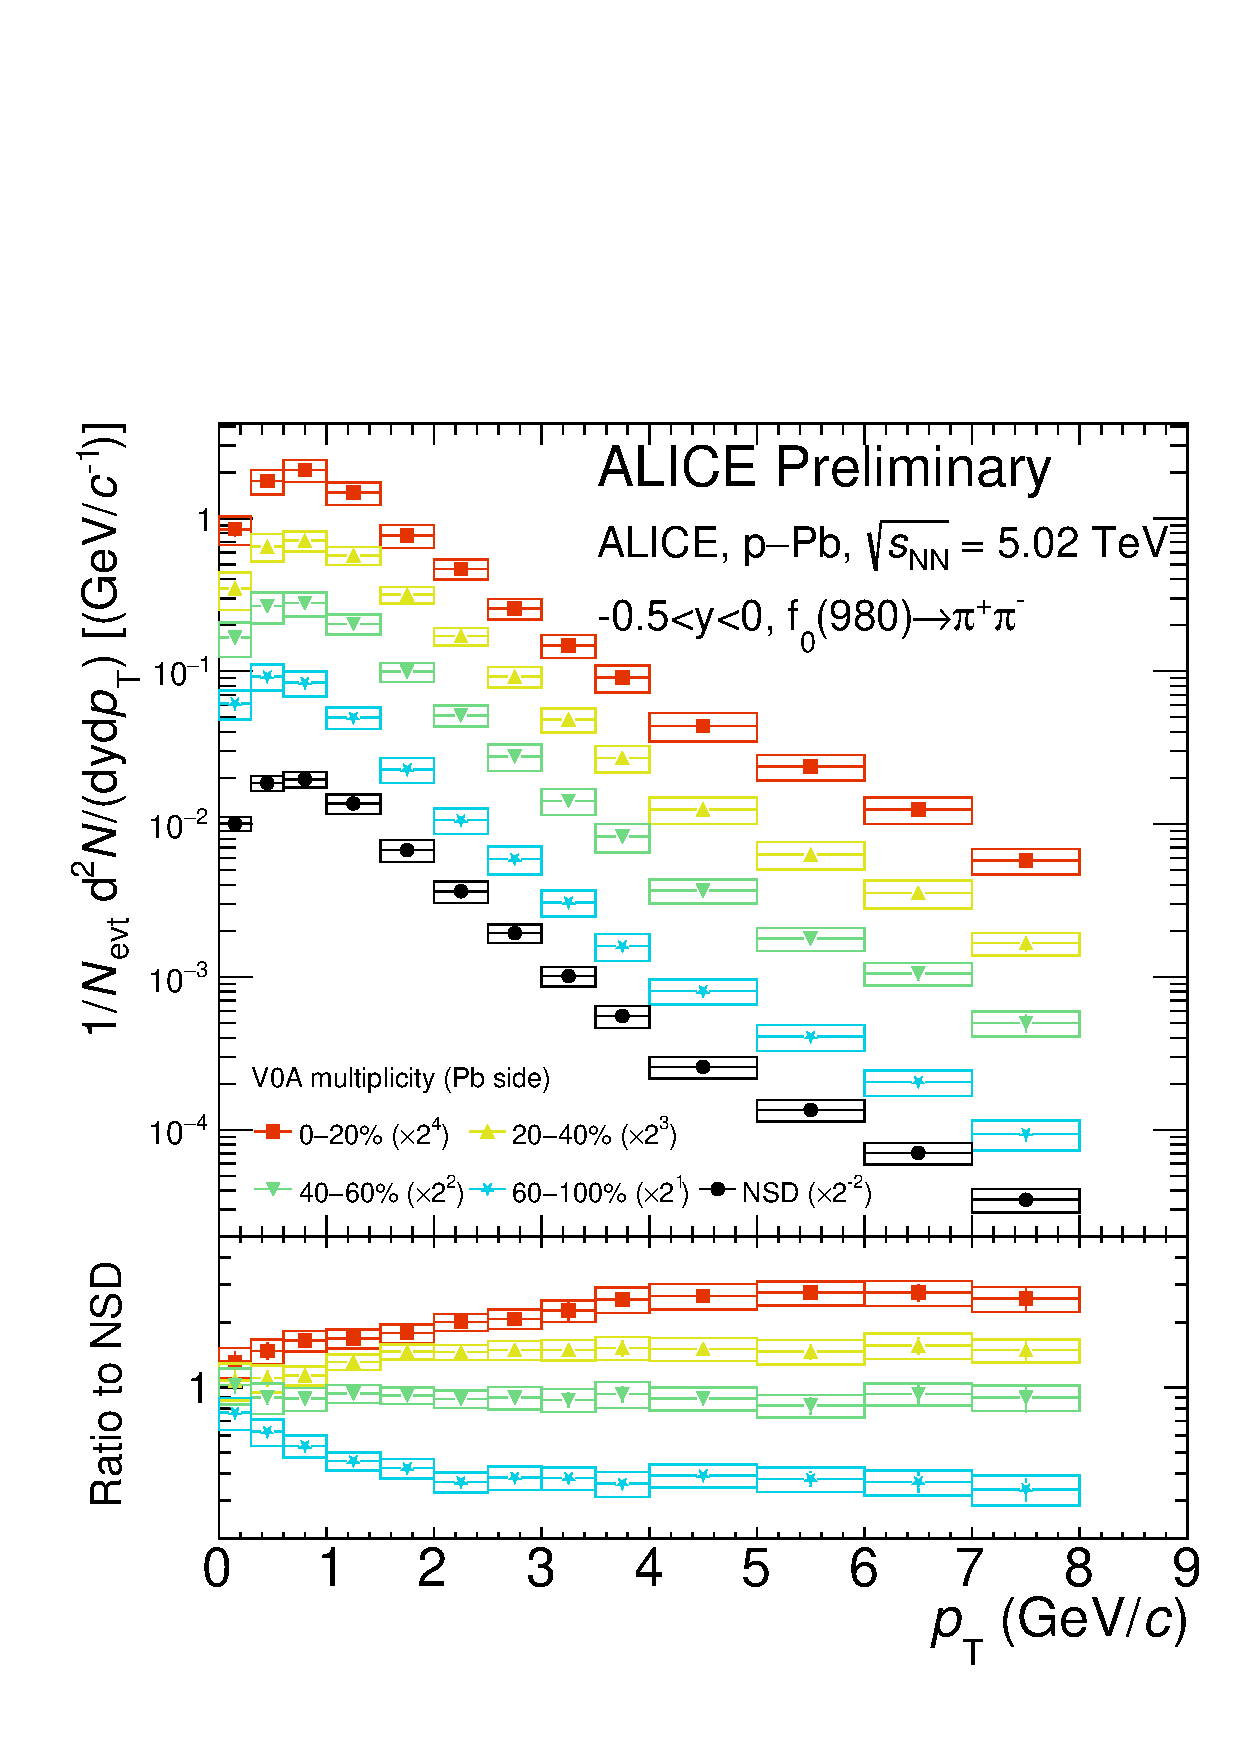
\includegraphics[width=0.6 \textwidth]{figures/Fig2_pt_all.pdf} }
	\caption{ Transverse momentum spectra of \fzero~in p--Pb collisions at \snn~=~5.02~TeV for different multiplicity classes, which are scaled for visibility. Statistical and systematic uncertainties are shown as error bars and boxes, respectively. The lower panel shows the ratios of the specific spectra to the NSD spectrum. }
	\label{fig:pt}
\end{figure}

Figure~\ref{fig:pt} shows the $p_{\mathrm{T}}$ spectra of \fzero~in p--Pb collisions at \snn~=~5.02~TeV measured in the range of 0~$<p_{\mathrm{T}}<$~8~GeV/$c$ for different multiplicity classes and non-single diffractive (NSD) events. Each spectrum is scaled with the number denoted in the figure for visibility. The lower panel of Fig.~\ref{fig:pt} shows the ratios of each $p_{\mathrm{T}}$ spectrum to the NSD spectrum. The systematic uncertainties of the ratios are estimated by propagating the multiplicity-uncorrelated uncertainties on the single spectrum. For $p_{\mathrm{T}}<$~4~GeV/$c$, the hardening of the $p_{\mathrm{T}}$ spectrum from low- to high-multiplicity events is clearly seen, while the same shape is visible at high $p_{\mathrm{T}}>$~4~GeV/$c$. Such trends can be also observed in other hadrons~\cite{Tsallis:1987eu}.

\begin{table}[h!]
\caption{The values of d$N$/d$y$ and mean $p_{\mathrm{T}}$ $\left( \left\langle p_{\mathrm{T}} \right\rangle \right)$ measured in p--Pb collisions at \snn~=~5.02~TeV for different multiplicity classes. The first and second uncertainties represent the statistical and systematic uncertainties, respectively. In each entry the first uncertainty is statistical and the second one is systematic. }
\centering
\begin{tabular}{ccc}
\hline 
Multiplicity class (V0A) & d$N$/dy & $\left\langle p_{\mathrm{T}} \right\rangle$ (GeV/$c$) \\ \hline
0--20\% & 0.206$\pm$0.005$\pm$0.014 & 1.287$\pm$0.034$\pm$0.010 \\
20--40\% & 0.153$\pm$0.004$\pm$0.010 & 1.250$\pm$0.029$\pm$0.082 \\
40--60\% & 0.113$\pm$0.002$\pm$0.008 & 1.142$\pm$0.025$\pm$0.088 \\
60--100\% & 0.064$\pm$0.001$\pm$0.005 & 0.999$\pm$0.014$\pm$0.080 \\
\hline
\end{tabular}
\label{tab:ymp}
\end{table}

Table~\ref{tab:ymp} shows the integrated yield (d$N$/d$y$) and mean $p_{\mathrm{T}}$ $\left( \left\langle p_{\mathrm{T}} \right\rangle \right)$ of \fzero~for different multiplicity classes in p--Pb collisions at \snn~=~5.02~TeV. The d$N$/d$y$ linearly increases with the multiplicity, while the $\left\langle p_{\mathrm{T}} \right\rangle$ concavely increases with the multiplicity. 

\begin{figure}[!hbt]
	\centering
	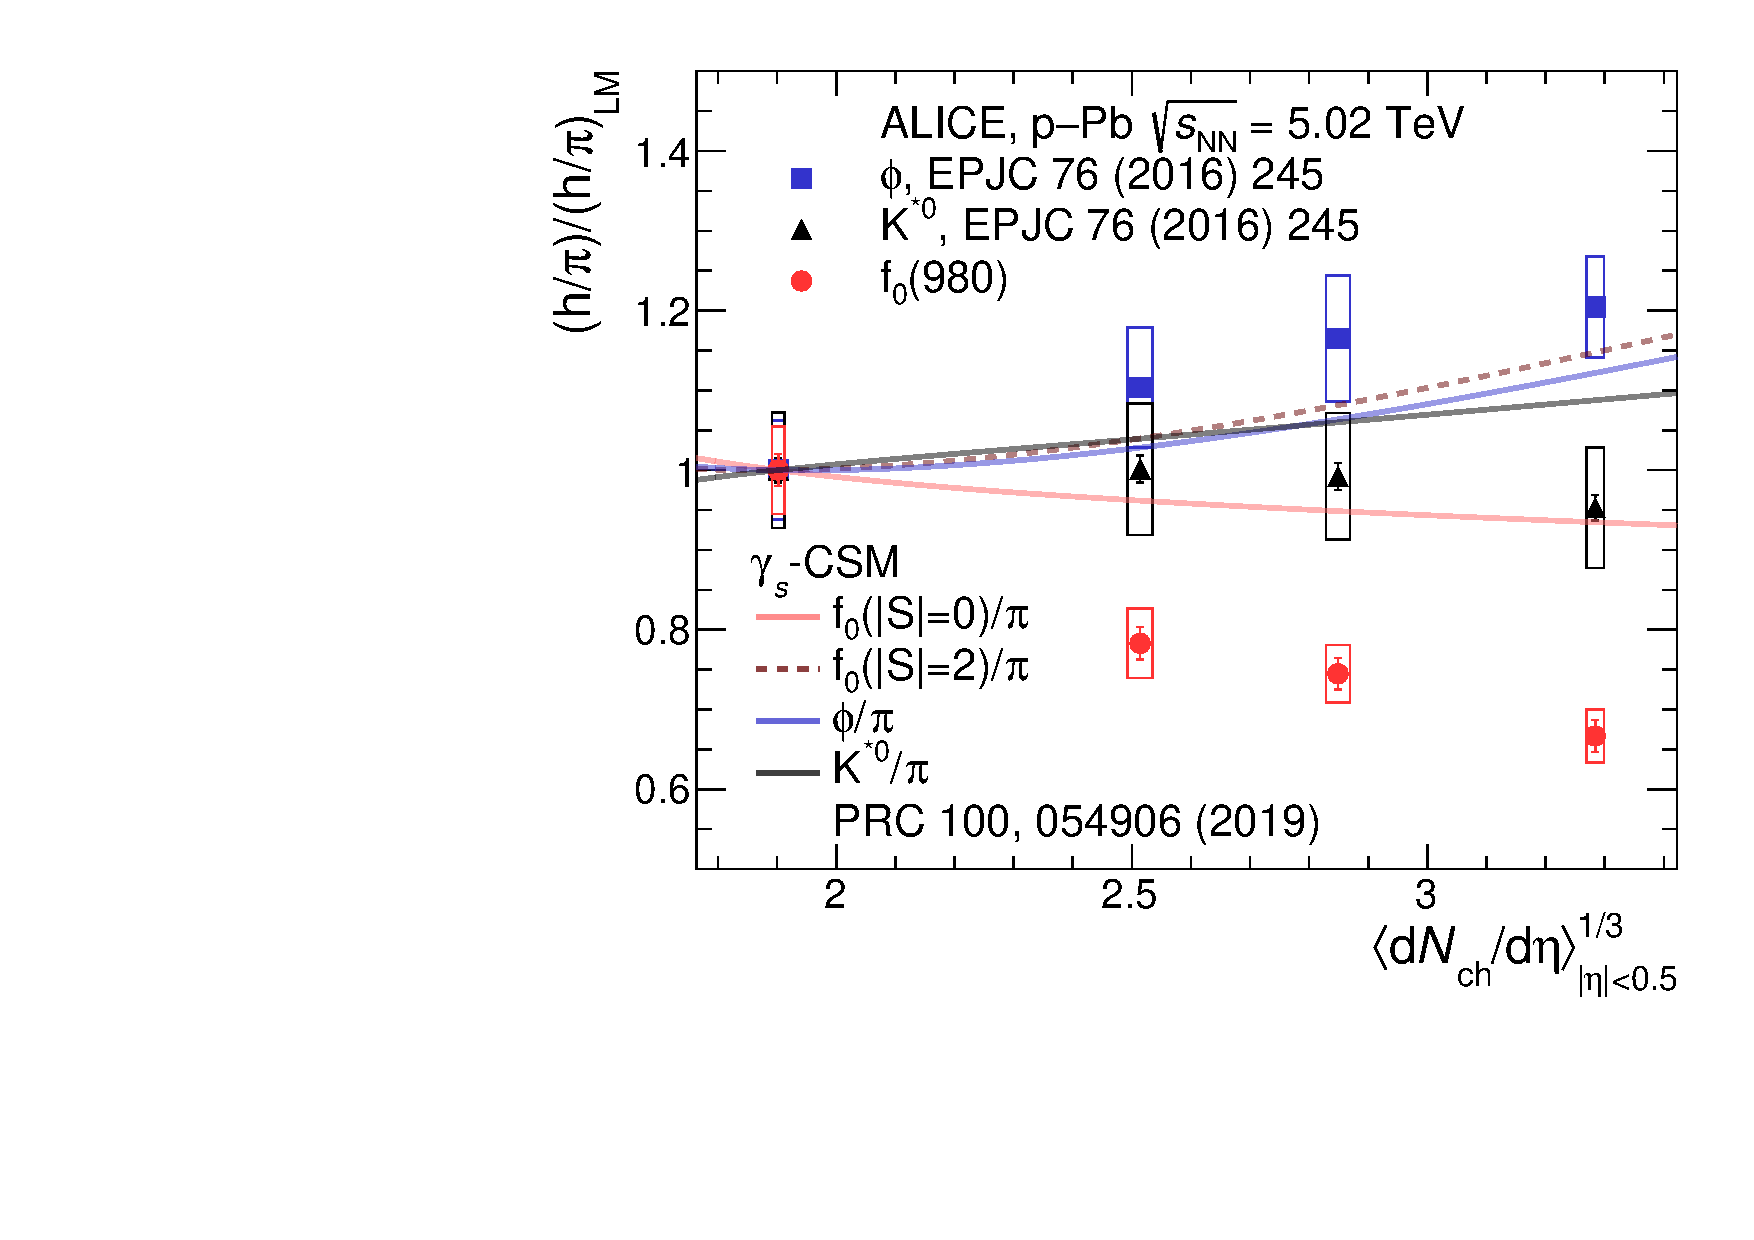
\includegraphics[width=0.49 \textwidth]{figures/Fig4_dr_pion_addCSM_addpar.pdf} 
        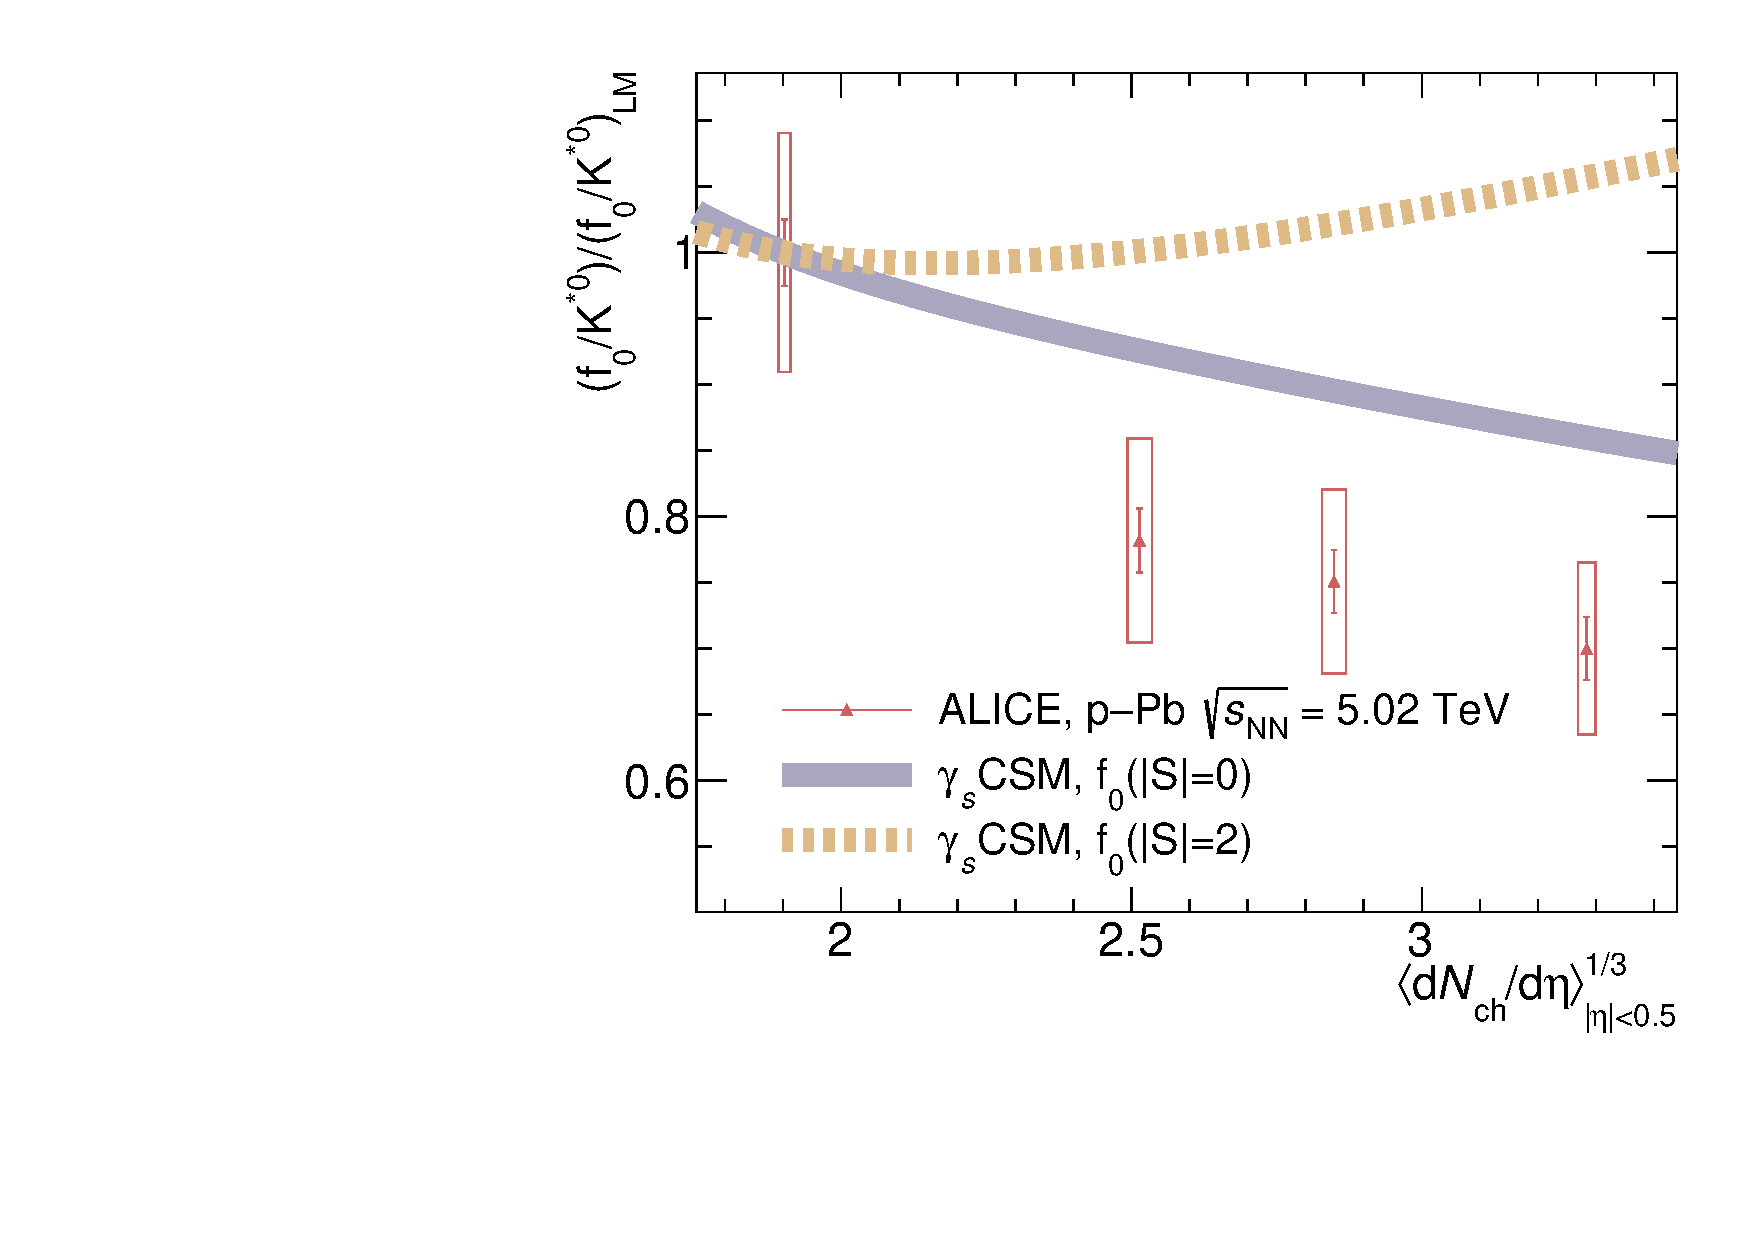
\includegraphics[width=0.49 \textwidth]{figures/Fig4_dr_kstar_addCSM.pdf} 
	\caption{ Double ratios of $\phi$, $\rm{}K^{*0}$(892), and \fzero~to $\pi$ (left) and \fzero~to $\rm{}K^{*0}$(892) (right) as a function of charged-particle multiplicity elevated to 1/3. The ratios are divided by the ratio in low-multiplicity (LM) events to make the first point unity and reduce systematic uncertainties. Predictions from the Canonical statistical model are represented with lines. }
	\label{fig:f0piAddCSM}
\end{figure}

The left panel of figure~\ref{fig:f0piAddCSM} shows the double ratios of different particles to charged pion yields as a function of charged-particle multiplicity elevated to 1/3 in p--Pb collisions at \snn~=~5.02~TeV. The charged-particle multiplicity is measured using the V0A detector. The systematic uncertainty of the double ratio is calculated with uncorrelated uncertainties only. The pion, $\rm{}K^{*0}$, and $\phi$ mesons can be classified according to their lifetimes and whether they contain (anti-) strange quarks. The strangeness enhancement and rescattering effects can be studied by comparing the yield of particles with different characteristics. The ratio of $\phi$ to $\pi$ increases with the multiplicity, which is consistent with the observation of the strangeness enhancement~\cite{ALICE:2016fzo}. On the other hand, the ratio of $\rm{}K^{*0}$ to $\pi$ is flat with the increasing multiplicity even if $\rm{}K^{*0}$ includes one strange quark. The flat trend could be explained by two competing effects, the strangeness enhancement and rescattering effects, as the lifetime of $\rm{}K^{*0}$ is 4.2~fm/$c$~\cite{ParticleDataGroup:2022pth}. The ratio of \fzero~to $\pi$ decreases as the multiplicity increases because of the shorter lifetime of \fzero, suggesting rescattering effects for \fzero. Predictions of the ratio of \fzero~to $\pi$ are shown in lines for different hidden strangeness assumptions for \fzero~by $\gamma_{s}$-Canonical Statistical Model (CSM)~\cite{Vovchenko:2019kes}, which considers system-size-dependent hadrochemistry at vanishing baryon density with local conservation of electric charge, baryon density, and strangeness, while allowing for undersaturation of strangeness. Note that $\gamma_{s}$ is the parameter for the undersaturation of strangeness derived from measured particle yields. The CSM hypothesis with 2 hidden strange quarks predicts an increase of the ratio, contrarily to what observed experimentally. Moreover, the CSM with zero hidden strangeness estimates the ratio to be flat, which overestimates the data. Such a difference is attributed to no rescattering effects in the CSM. The prediction of the CSM for the ratio of $\phi$ to $\pi$ nicely reproduces the increasing trend of measured data with the increasing multiplicity. However, the CSM overestimates the ratio of $\rm{}K^{*0}$ to $\pi$ because the modification of $\rm{}K^{*0}$ yields due to rescattering effects is not implemented in the CSM.

The right panel of figure~\ref{fig:f0piAddCSM} shows the double ratio of \fzero~to $\rm{}K^{*0}$ yields as a function of charged-particle multiplicity elevated to 1/3 in p--Pb collisions at \snn~=~5.02~TeV and predictions from the CSM with different hidden strangeness assumptions. The lifetimes of \fzero~and $\rm{}K^{*0}$ are estimated to be comparable, indicating that rescattering effects would not be much different. Hence, the ratio is expected to be weakly affected by rescattering effects. The ratio decreases with increasing multiplicity that is qualitatively described with the zero-hidden-strangeness assumption and can be explained by the strangeness enhancement of the $\rm{}K^{*0}$ yield. The CSM prediction with the two-hidden-strangeness assumptions is mildly increasing as the multiplicity increases, a trend that is opposite to the experimental result as shown in Fig.~\ref{fig:f0piAddCSM}. Therefore, the decreasing trend of the ratio of \fzero~to $\rm{}K^{*0}$ can suggest no effective strangeness enhancement for the \fzero.

\begin{figure}[!hbt]
	\centering
	\subfigure{ 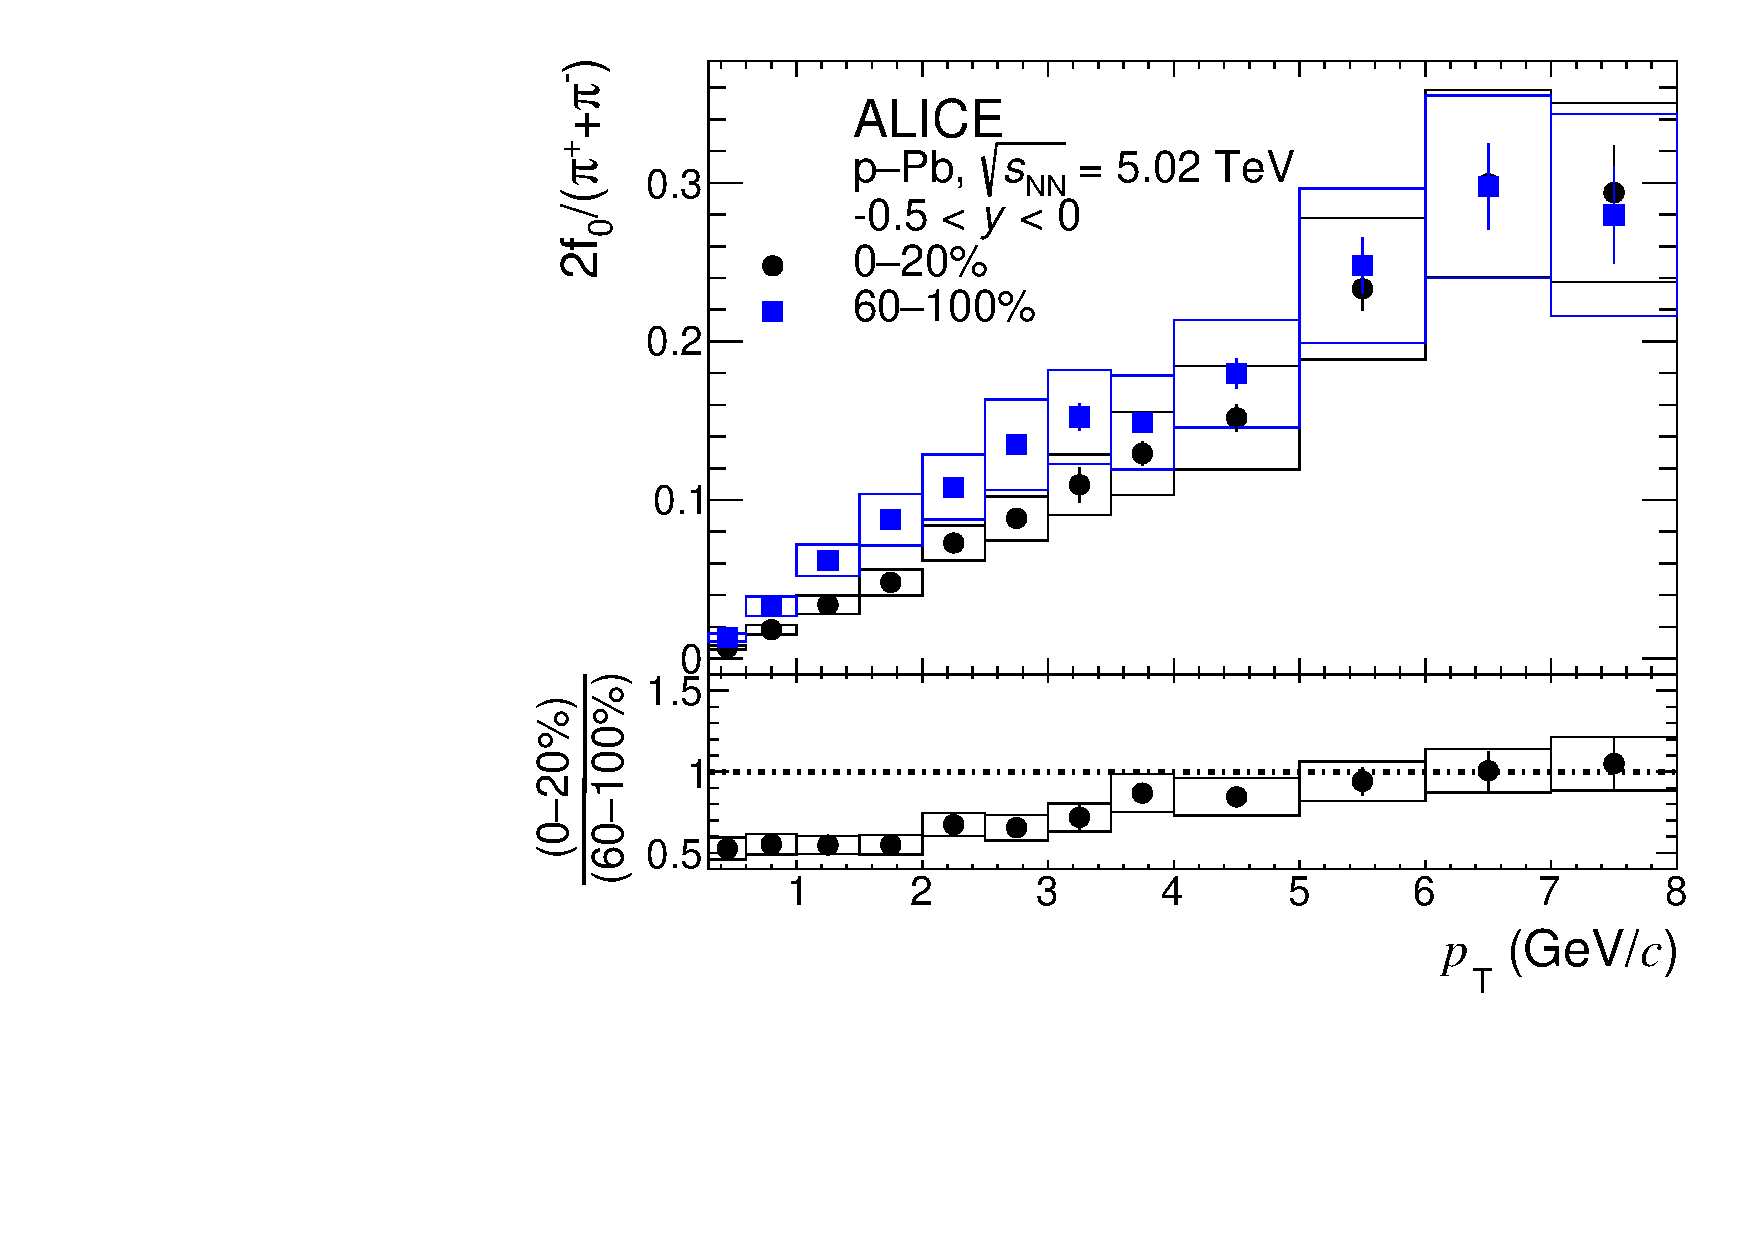
\includegraphics[width=0.6 \textwidth]{figures/Fig5_DR_pt_pion.pdf} }
	\caption{ The particle yield ratios of \fzero~to $\pi$ as a function of $p_{\rm{T}}$ in high-multiplicity (circles) and low-multiplicity (triangles) p--Pb collisions at \snn~=~5.02~TeV. The lower panel shows the double ratio of \fzero/$\pi$ between the high-multiplicity and low-multiplicity events. }
	\label{fig:f0piPt}
\end{figure}

Figure~\ref{fig:f0piPt} shows the $p_{\mathrm{T}}$-differential particle yield ratio of \fzero~to $\pi$ in high-multiplicity (HM) and low-multiplicity (LM) p--Pb collisions at \snn~=~5.02~TeV. The ratios are consistent within one sigma in $p_{\mathrm{T}}>$~4~GeV/$c$, while the double ratio of HM to LM is suppressed at a lower $p_{\mathrm{T}}$ as shown in the lower panel of Fig.~\ref{fig:f0piPt}. In the double ratio, the correlated uncertainties across multiplicity classes cancel. The $p_{\mathrm{T}}$ dependence of the double ratio indicates that the suppression of the integrated yield is an effect of the low $p_{\mathrm{T}}$ ($p_{\mathrm{T}}<$~4~GeV/$c$), which shows the same $p_{\mathrm{T}}$ dependence like the suppression of the $\rm{}K^{*0}/K$~\cite{ALICE:2019etb}.

\begin{figure}[!hbt]
	\centering
	\subfigure{ 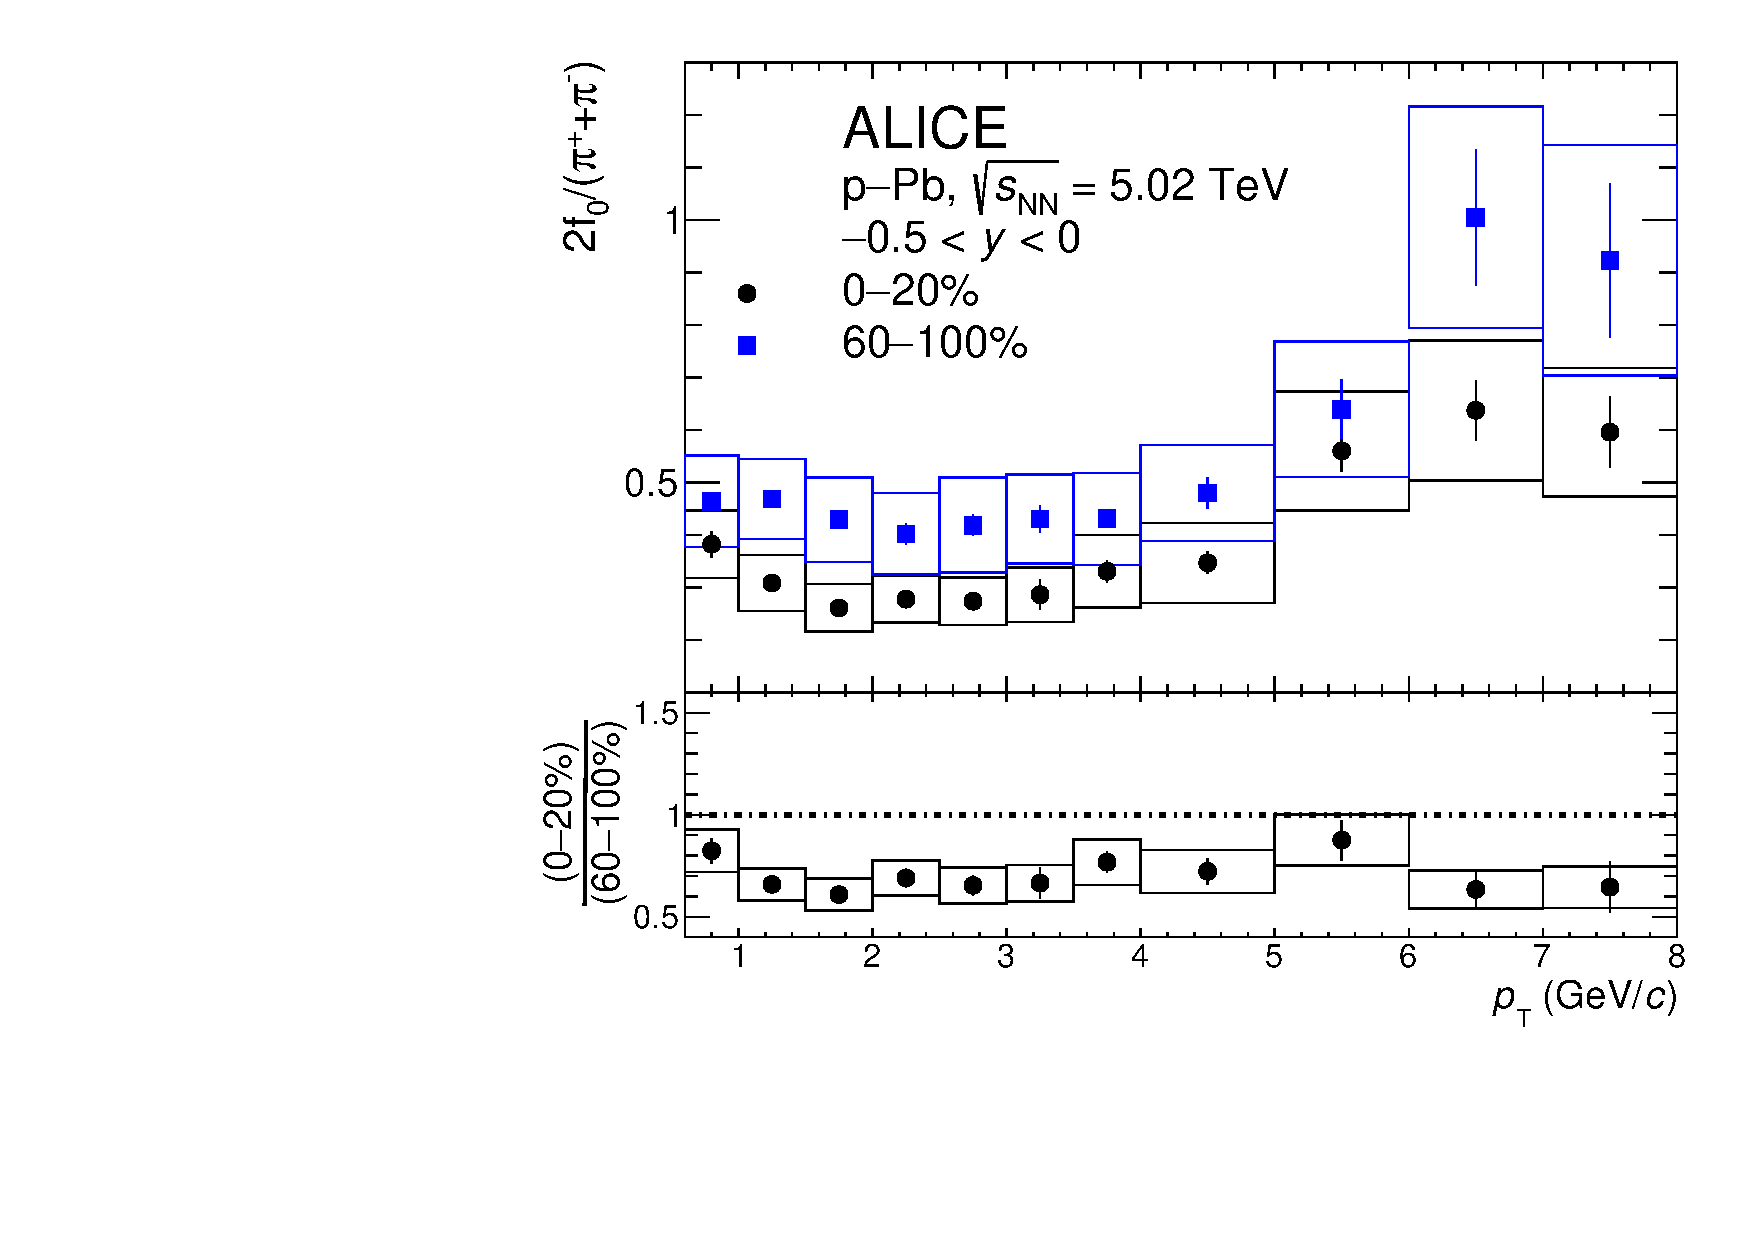
\includegraphics[width=0.6 \textwidth]{figures/Fig6_DR_pt_kstar.pdf} }
	\caption{The particle yield ratio of \fzero~to $\rm{}K^{*0}$(892) as a function of $p_{\rm{T}}$ in high-multiplicity (circles) and low-multiplicity (triangles) p--Pb collisions at \snn~=~5.02~TeV. The lower panel shows the double ratio of high-multiplicity to low-multiplicity \fzero/$\rm{}K^{*0}$(892).  }
	\label{fig:f0KsPt}
\end{figure}

Figure~\ref{fig:f0KsPt} shows $p_{\mathrm{T}}$-differential particle yield ratio of \fzero~to $\rm{}K^{*0}$ in HM and LM p--Pb collisions at \snn~=~5.02~TeV. The ratio from HM events is lower than that of LM events in the entire $p_{\mathrm{T}}$ range, which is different from $\rm{}K^{*0}/K$ or \fzero/$\pi$. The different $p_{\mathrm{T}}$ dependence of the double ratio indicates that other effects, rather than rescattering effects, are present. For instance, the enhancement of $\rm{}K^{*0}$ yield due to the strangeness enhancement can explain the suppression in the entire $p_{\mathrm{T}}$ range, while no strangeness enhancement for \fzero~yield. As a result, the decreasing trend of the ratio in higher multiplicity events suggests no strange quark in \fzero.

\begin{figure}[!hbt]
	\centering
	\subfigure{ 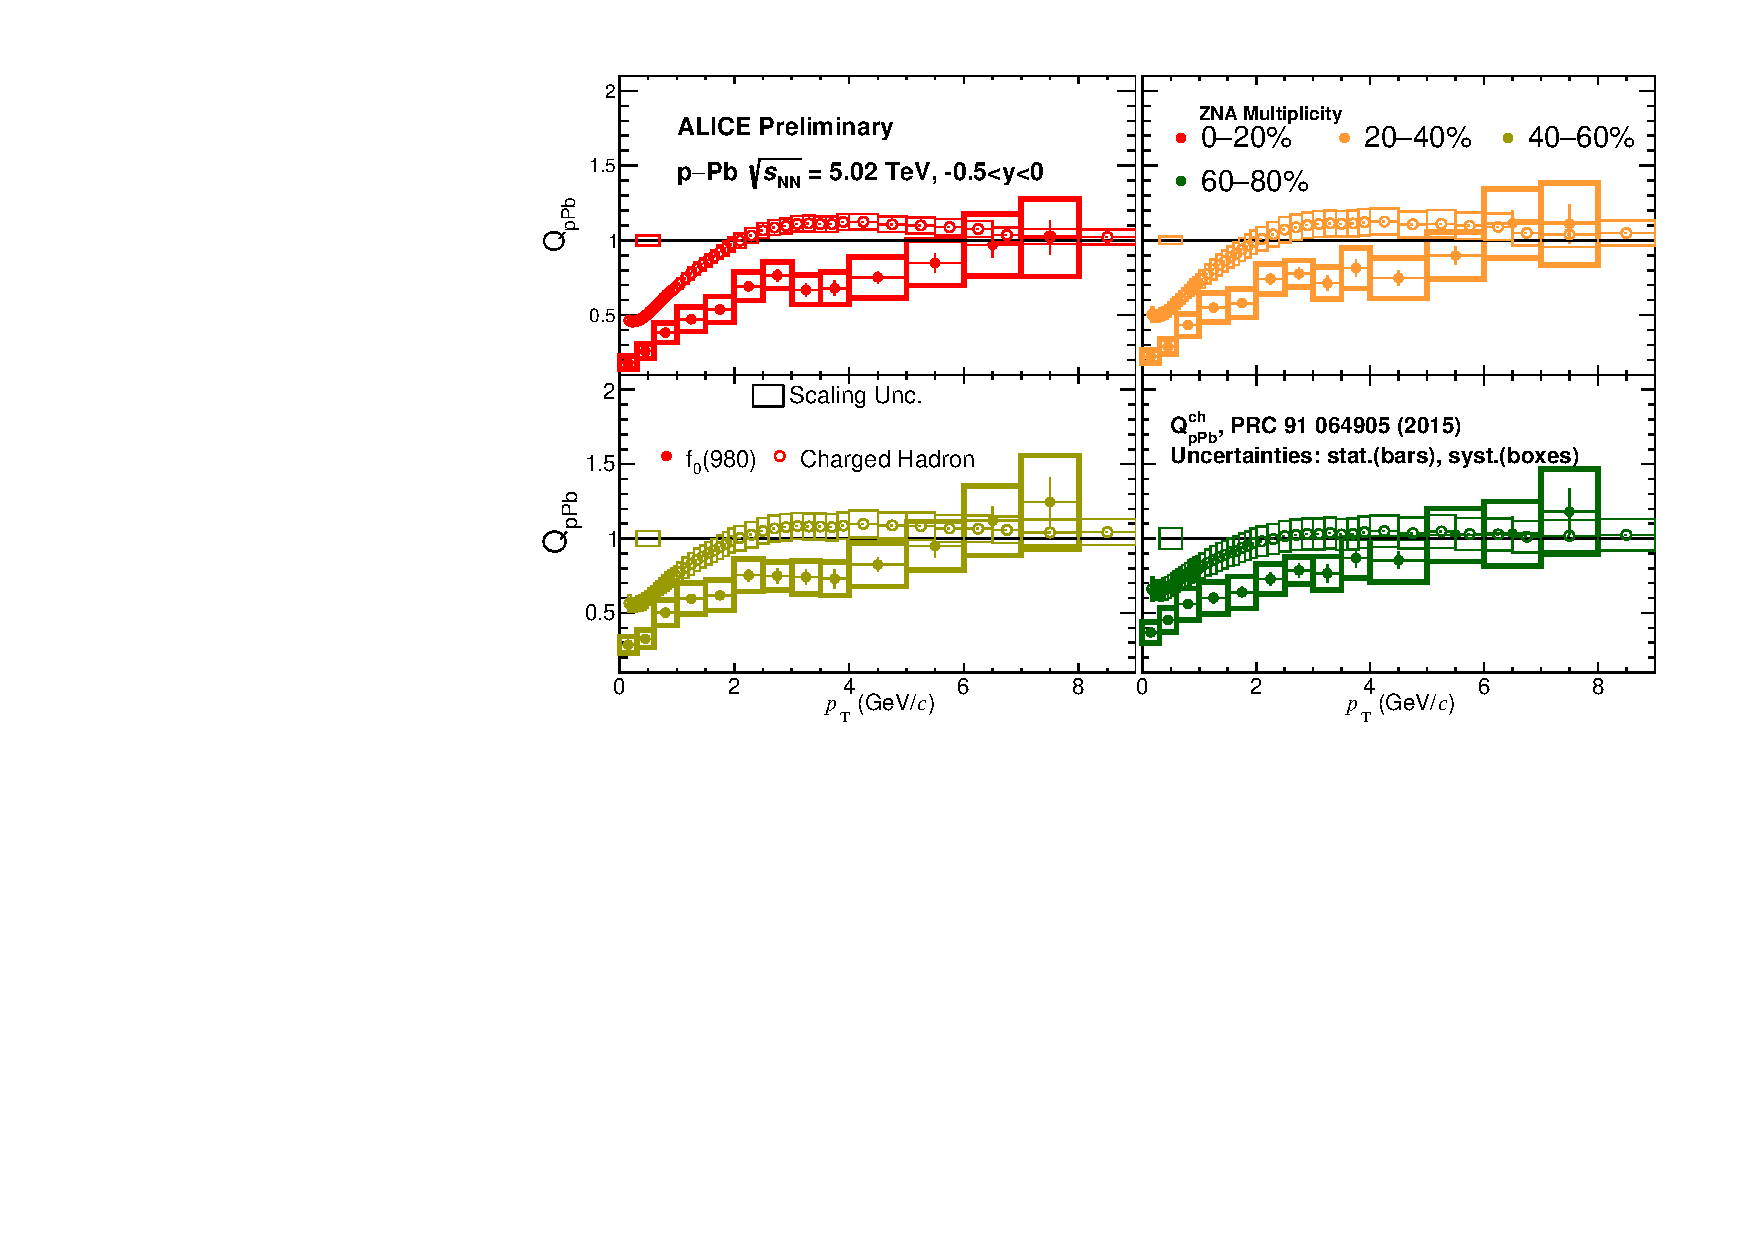
\includegraphics[width=0.8 \textwidth]{figures/Fig7_QpPb.pdf} }
	\caption{ Nuclear modification factor ($Q_{\rm{pPb}}$) of \fzero~as a function of $p_{\rm{T}}$ in p--Pb collisions at \snn~=~5.02~TeV for different multiplicity classes. Statistical and systematic uncertainties are shown as error bars and boxes, respectively. Open boxes around $p_{\rm{T}}$~=~0.5~GeV/$c$ represent the binary collision scaling uncertainties. The $Q_{\rm{pPb}}$ of \fzero~is compared with $Q_{\rm{pPb}}$~of charged hadrons. }
	\label{fig:QpPb}
\end{figure}

The $p_{\rm{T}}$-differential invariant yield of \fzero in p--Pb collisions can be compared to the one in pp collisions at the same center-of-mass energy by computing the nuclear modification factor $Q_{\mbox{pPb}}$, defined as 
\begin{eqnarray}
Q_{\mbox{pPb}} = \dfrac{\mathrm{d}^{2} N_{\mathrm{f}_{0}(980)}^{\mathrm{pPb}} / \mathrm{d} p_{\mathrm{T}} \mathrm{dy} }{ \left\langle T_{\mathrm{pPb}} \right\rangle \mathrm{d}^{2} \sigma_{\mathrm{f}_{0}(980)}^{\mathrm{pp}}/ \mathrm{d} p_{\mathrm{T}} \mathrm{dy} },
\end{eqnarray}
where $\left\langle T_{\mathrm{pPb}} \right\rangle$ and $\sigma_{\mathrm{f}_{0}(980)}^{\mathrm{pp}}$ are the average nuclear overlap from the Glauber model~\cite{Miller:2007ri} and the cross section for the production of \fzero~in pp collisions~\cite{ALICE:2022qnb}, respectively. Note that the B.R. is cancelled out in the measurement of the $Q_{\mbox{pPb}}$ as the same value is used in pp and p--Pb collisions.

Figure~\ref{fig:QpPb} shows the $Q_{\mbox{pPb}}$ of \fzero~in p--Pb collisions at \snn~=~5.02~TeV in different multiplicity classes. The Pb-remnant side ZN is used to select centrality intervals to calculate the $Q_{\mathrm{pPb}}$, which is described in Sec.~\ref{sec:setup}. The systematic uncertainties are calculated with the assumption that there is no correlated uncertainty between the yield in pp and p--Pb collisions. The \fzero~is more suppressed than charged hadrons in all measured centrality intervals for $p_{\mathrm{T}}<$~4~GeV/$c$. As $p_{\mathrm{T}}$ increases, $Q_{\rm{pPb}}$ becomes compatible and reaches unity for both cases. This result is consistent with the suppression shown in Fig.~\ref{fig:f0piPt}, indicating the strong suppression at low $p_{\mathrm{T}}$ and no suppression observed at high $p_{\mathrm{T}}$. In addition, the $Q_{\rm{pPb}}$ does not exhibit Cronin peak~\cite{Cronin:1974zm} at the intermediate $p_{\mathrm{T}}$ in HM events. This is consistent trend of conventional mesons. No Cronin peak for \fzero~might suggests that the number of constituent quarks of \fzero~is smaller than three.
% !TEX root = paper.tex

\section{Conclusions}
\label{sec:summary}

The multiplicity dependent \fzero~production in p--Pb collisions at \snn~=~5.02~TeV is presented. \fzero~is reconstructed via the \fzero~$\rightarrow\pi^{+}\pi^{-}$ decay channel in midrapidity (-0.5~$<y<$~0) in the transverse momentum region of $0<p_{\mathrm{T}}<8$~GeV/$c$.
The transverse momentum ($p_{\mathrm{T}}$) spectra of \fzero~ particles show an increasing trend of the yield and the mean $p_{\mathrm{T}}$ for higher multiplicity events. The particle yield ratio of \fzero~to $\pi$ is decreasing with the multiplicity and the suppression exists only at low $p_{\mathrm{T}}<$~4~GeV/$c$, indicating that the rescattering effects exist for \fzero~particles. The Canonical Statistical Model (CSM) overestimates the \fzero/$\pi$ and it does not describe the decreasing trend because the CSM does not consider rescattering effects. The particle yield ratio of \fzero~to $\rm{}K^{*0}$ also decreases with the increasing multiplicity. The suppression exists in the entire $p_{\mathrm{T}}$ range, which is a different $p_{\mathrm{T}}$ dependency from rescattering effects. The CSM qualitatively estimates the decreasing trend for \fzero/$\rm{}K^{*0}$ with the assumption of no hidden strangeness for \fzero, while it overestimates the \fzero/$\rm{}K^{*0}$ with the assumption of the two hidden strangeness. The result implies that $\rm{}K^{*0}$ is relatively enhanced compared with \fzero~due to the strangeness enhancement. Furthermore, the multiplicity-dependent nuclear modification factor for \fzero~exhibits a strong suppression at a low $p_{\mathrm{T}}$ and the suppression depends on the multiplicity class, which can be explained by the rescattering effects. Additionally, no Cronin peak is observed from the nuclear modification factor, even in high-multiplicity events. This suggests the number of constituent quarks of the \fzero~particle is smaller than three.



%%%%% acknowledgements
\newenvironment{acknowledgement}{\relax}{\relax}
\begin{acknowledgement}
\section*{Acknowledgements}
\noindent 
%{\it (TBI: The default acknowledgments will be done by EB centrally.)}
%\input{acknowledgements.tex}    %%%%%%% done by webmaster team
\end{acknowledgement}

\newpage
\appendix



\clearpage

\bibliographystyle{utphys}
\bibliography{paper.bib}

%%%%%%%%% appendix with author list
%\section{The ALICE Collaboration}
%\label{app:collab}
%\input{Alice_Authorlist_2017-Aug-21.tex}  %%%%%%% done by webmaster team
%\input{}     


\end{document}
